
% Default to the notebook output style

    


% Inherit from the specified cell style.




    
\documentclass{article}

    
    
    \usepackage{graphicx} % Used to insert images
    \usepackage{adjustbox} % Used to constrain images to a maximum size 
    \usepackage{color} % Allow colors to be defined
    \usepackage{enumerate} % Needed for markdown enumerations to work
    \usepackage{geometry} % Used to adjust the document margins
    \usepackage{amsmath} % Equations
    \usepackage{amssymb} % Equations
    \usepackage[mathletters]{ucs} % Extended unicode (utf-8) support
    \usepackage[utf8x]{inputenc} % Allow utf-8 characters in the tex document
    \usepackage{fancyvrb} % verbatim replacement that allows latex
    \usepackage{grffile} % extends the file name processing of package graphics 
                         % to support a larger range 
    % The hyperref package gives us a pdf with properly built
    % internal navigation ('pdf bookmarks' for the table of contents,
    % internal cross-reference links, web links for URLs, etc.)
    \usepackage{hyperref}
    \usepackage{longtable} % longtable support required by pandoc >1.10
    \usepackage{booktabs}  % table support for pandoc > 1.12.2
    

    
    
    \definecolor{orange}{cmyk}{0,0.4,0.8,0.2}
    \definecolor{darkorange}{rgb}{.71,0.21,0.01}
    \definecolor{darkgreen}{rgb}{.12,.54,.11}
    \definecolor{myteal}{rgb}{.26, .44, .56}
    \definecolor{gray}{gray}{0.45}
    \definecolor{lightgray}{gray}{.95}
    \definecolor{mediumgray}{gray}{.8}
    \definecolor{inputbackground}{rgb}{.95, .95, .85}
    \definecolor{outputbackground}{rgb}{.95, .95, .95}
    \definecolor{traceback}{rgb}{1, .95, .95}
    % ansi colors
    \definecolor{red}{rgb}{.6,0,0}
    \definecolor{green}{rgb}{0,.65,0}
    \definecolor{brown}{rgb}{0.6,0.6,0}
    \definecolor{blue}{rgb}{0,.145,.698}
    \definecolor{purple}{rgb}{.698,.145,.698}
    \definecolor{cyan}{rgb}{0,.698,.698}
    \definecolor{lightgray}{gray}{0.5}
    
    % bright ansi colors
    \definecolor{darkgray}{gray}{0.25}
    \definecolor{lightred}{rgb}{1.0,0.39,0.28}
    \definecolor{lightgreen}{rgb}{0.48,0.99,0.0}
    \definecolor{lightblue}{rgb}{0.53,0.81,0.92}
    \definecolor{lightpurple}{rgb}{0.87,0.63,0.87}
    \definecolor{lightcyan}{rgb}{0.5,1.0,0.83}
    
    % commands and environments needed by pandoc snippets
    % extracted from the output of `pandoc -s`
    \DefineVerbatimEnvironment{Highlighting}{Verbatim}{commandchars=\\\{\}}
    % Add ',fontsize=\small' for more characters per line
    \newenvironment{Shaded}{}{}
    \newcommand{\KeywordTok}[1]{\textcolor[rgb]{0.00,0.44,0.13}{\textbf{{#1}}}}
    \newcommand{\DataTypeTok}[1]{\textcolor[rgb]{0.56,0.13,0.00}{{#1}}}
    \newcommand{\DecValTok}[1]{\textcolor[rgb]{0.25,0.63,0.44}{{#1}}}
    \newcommand{\BaseNTok}[1]{\textcolor[rgb]{0.25,0.63,0.44}{{#1}}}
    \newcommand{\FloatTok}[1]{\textcolor[rgb]{0.25,0.63,0.44}{{#1}}}
    \newcommand{\CharTok}[1]{\textcolor[rgb]{0.25,0.44,0.63}{{#1}}}
    \newcommand{\StringTok}[1]{\textcolor[rgb]{0.25,0.44,0.63}{{#1}}}
    \newcommand{\CommentTok}[1]{\textcolor[rgb]{0.38,0.63,0.69}{\textit{{#1}}}}
    \newcommand{\OtherTok}[1]{\textcolor[rgb]{0.00,0.44,0.13}{{#1}}}
    \newcommand{\AlertTok}[1]{\textcolor[rgb]{1.00,0.00,0.00}{\textbf{{#1}}}}
    \newcommand{\FunctionTok}[1]{\textcolor[rgb]{0.02,0.16,0.49}{{#1}}}
    \newcommand{\RegionMarkerTok}[1]{{#1}}
    \newcommand{\ErrorTok}[1]{\textcolor[rgb]{1.00,0.00,0.00}{\textbf{{#1}}}}
    \newcommand{\NormalTok}[1]{{#1}}
    
    % Define a nice break command that doesn't care if a line doesn't already
    % exist.
    \def\br{\hspace*{\fill} \\* }
    % Math Jax compatability definitions
    \def\gt{>}
    \def\lt{<}
    % Document parameters
    \title{01\_Introducing\_Python}
    
    
    

    % Pygments definitions
    
\makeatletter
\def\PY@reset{\let\PY@it=\relax \let\PY@bf=\relax%
    \let\PY@ul=\relax \let\PY@tc=\relax%
    \let\PY@bc=\relax \let\PY@ff=\relax}
\def\PY@tok#1{\csname PY@tok@#1\endcsname}
\def\PY@toks#1+{\ifx\relax#1\empty\else%
    \PY@tok{#1}\expandafter\PY@toks\fi}
\def\PY@do#1{\PY@bc{\PY@tc{\PY@ul{%
    \PY@it{\PY@bf{\PY@ff{#1}}}}}}}
\def\PY#1#2{\PY@reset\PY@toks#1+\relax+\PY@do{#2}}

\expandafter\def\csname PY@tok@gd\endcsname{\def\PY@tc##1{\textcolor[rgb]{0.63,0.00,0.00}{##1}}}
\expandafter\def\csname PY@tok@gu\endcsname{\let\PY@bf=\textbf\def\PY@tc##1{\textcolor[rgb]{0.50,0.00,0.50}{##1}}}
\expandafter\def\csname PY@tok@gt\endcsname{\def\PY@tc##1{\textcolor[rgb]{0.00,0.27,0.87}{##1}}}
\expandafter\def\csname PY@tok@gs\endcsname{\let\PY@bf=\textbf}
\expandafter\def\csname PY@tok@gr\endcsname{\def\PY@tc##1{\textcolor[rgb]{1.00,0.00,0.00}{##1}}}
\expandafter\def\csname PY@tok@cm\endcsname{\let\PY@it=\textit\def\PY@tc##1{\textcolor[rgb]{0.25,0.50,0.50}{##1}}}
\expandafter\def\csname PY@tok@vg\endcsname{\def\PY@tc##1{\textcolor[rgb]{0.10,0.09,0.49}{##1}}}
\expandafter\def\csname PY@tok@m\endcsname{\def\PY@tc##1{\textcolor[rgb]{0.40,0.40,0.40}{##1}}}
\expandafter\def\csname PY@tok@mh\endcsname{\def\PY@tc##1{\textcolor[rgb]{0.40,0.40,0.40}{##1}}}
\expandafter\def\csname PY@tok@go\endcsname{\def\PY@tc##1{\textcolor[rgb]{0.53,0.53,0.53}{##1}}}
\expandafter\def\csname PY@tok@ge\endcsname{\let\PY@it=\textit}
\expandafter\def\csname PY@tok@vc\endcsname{\def\PY@tc##1{\textcolor[rgb]{0.10,0.09,0.49}{##1}}}
\expandafter\def\csname PY@tok@il\endcsname{\def\PY@tc##1{\textcolor[rgb]{0.40,0.40,0.40}{##1}}}
\expandafter\def\csname PY@tok@cs\endcsname{\let\PY@it=\textit\def\PY@tc##1{\textcolor[rgb]{0.25,0.50,0.50}{##1}}}
\expandafter\def\csname PY@tok@cp\endcsname{\def\PY@tc##1{\textcolor[rgb]{0.74,0.48,0.00}{##1}}}
\expandafter\def\csname PY@tok@gi\endcsname{\def\PY@tc##1{\textcolor[rgb]{0.00,0.63,0.00}{##1}}}
\expandafter\def\csname PY@tok@gh\endcsname{\let\PY@bf=\textbf\def\PY@tc##1{\textcolor[rgb]{0.00,0.00,0.50}{##1}}}
\expandafter\def\csname PY@tok@ni\endcsname{\let\PY@bf=\textbf\def\PY@tc##1{\textcolor[rgb]{0.60,0.60,0.60}{##1}}}
\expandafter\def\csname PY@tok@nl\endcsname{\def\PY@tc##1{\textcolor[rgb]{0.63,0.63,0.00}{##1}}}
\expandafter\def\csname PY@tok@nn\endcsname{\let\PY@bf=\textbf\def\PY@tc##1{\textcolor[rgb]{0.00,0.00,1.00}{##1}}}
\expandafter\def\csname PY@tok@no\endcsname{\def\PY@tc##1{\textcolor[rgb]{0.53,0.00,0.00}{##1}}}
\expandafter\def\csname PY@tok@na\endcsname{\def\PY@tc##1{\textcolor[rgb]{0.49,0.56,0.16}{##1}}}
\expandafter\def\csname PY@tok@nb\endcsname{\def\PY@tc##1{\textcolor[rgb]{0.00,0.50,0.00}{##1}}}
\expandafter\def\csname PY@tok@nc\endcsname{\let\PY@bf=\textbf\def\PY@tc##1{\textcolor[rgb]{0.00,0.00,1.00}{##1}}}
\expandafter\def\csname PY@tok@nd\endcsname{\def\PY@tc##1{\textcolor[rgb]{0.67,0.13,1.00}{##1}}}
\expandafter\def\csname PY@tok@ne\endcsname{\let\PY@bf=\textbf\def\PY@tc##1{\textcolor[rgb]{0.82,0.25,0.23}{##1}}}
\expandafter\def\csname PY@tok@nf\endcsname{\def\PY@tc##1{\textcolor[rgb]{0.00,0.00,1.00}{##1}}}
\expandafter\def\csname PY@tok@si\endcsname{\let\PY@bf=\textbf\def\PY@tc##1{\textcolor[rgb]{0.73,0.40,0.53}{##1}}}
\expandafter\def\csname PY@tok@s2\endcsname{\def\PY@tc##1{\textcolor[rgb]{0.73,0.13,0.13}{##1}}}
\expandafter\def\csname PY@tok@vi\endcsname{\def\PY@tc##1{\textcolor[rgb]{0.10,0.09,0.49}{##1}}}
\expandafter\def\csname PY@tok@nt\endcsname{\let\PY@bf=\textbf\def\PY@tc##1{\textcolor[rgb]{0.00,0.50,0.00}{##1}}}
\expandafter\def\csname PY@tok@nv\endcsname{\def\PY@tc##1{\textcolor[rgb]{0.10,0.09,0.49}{##1}}}
\expandafter\def\csname PY@tok@s1\endcsname{\def\PY@tc##1{\textcolor[rgb]{0.73,0.13,0.13}{##1}}}
\expandafter\def\csname PY@tok@sh\endcsname{\def\PY@tc##1{\textcolor[rgb]{0.73,0.13,0.13}{##1}}}
\expandafter\def\csname PY@tok@sc\endcsname{\def\PY@tc##1{\textcolor[rgb]{0.73,0.13,0.13}{##1}}}
\expandafter\def\csname PY@tok@sx\endcsname{\def\PY@tc##1{\textcolor[rgb]{0.00,0.50,0.00}{##1}}}
\expandafter\def\csname PY@tok@bp\endcsname{\def\PY@tc##1{\textcolor[rgb]{0.00,0.50,0.00}{##1}}}
\expandafter\def\csname PY@tok@c1\endcsname{\let\PY@it=\textit\def\PY@tc##1{\textcolor[rgb]{0.25,0.50,0.50}{##1}}}
\expandafter\def\csname PY@tok@kc\endcsname{\let\PY@bf=\textbf\def\PY@tc##1{\textcolor[rgb]{0.00,0.50,0.00}{##1}}}
\expandafter\def\csname PY@tok@c\endcsname{\let\PY@it=\textit\def\PY@tc##1{\textcolor[rgb]{0.25,0.50,0.50}{##1}}}
\expandafter\def\csname PY@tok@mf\endcsname{\def\PY@tc##1{\textcolor[rgb]{0.40,0.40,0.40}{##1}}}
\expandafter\def\csname PY@tok@err\endcsname{\def\PY@bc##1{\setlength{\fboxsep}{0pt}\fcolorbox[rgb]{1.00,0.00,0.00}{1,1,1}{\strut ##1}}}
\expandafter\def\csname PY@tok@kd\endcsname{\let\PY@bf=\textbf\def\PY@tc##1{\textcolor[rgb]{0.00,0.50,0.00}{##1}}}
\expandafter\def\csname PY@tok@ss\endcsname{\def\PY@tc##1{\textcolor[rgb]{0.10,0.09,0.49}{##1}}}
\expandafter\def\csname PY@tok@sr\endcsname{\def\PY@tc##1{\textcolor[rgb]{0.73,0.40,0.53}{##1}}}
\expandafter\def\csname PY@tok@mo\endcsname{\def\PY@tc##1{\textcolor[rgb]{0.40,0.40,0.40}{##1}}}
\expandafter\def\csname PY@tok@kn\endcsname{\let\PY@bf=\textbf\def\PY@tc##1{\textcolor[rgb]{0.00,0.50,0.00}{##1}}}
\expandafter\def\csname PY@tok@mi\endcsname{\def\PY@tc##1{\textcolor[rgb]{0.40,0.40,0.40}{##1}}}
\expandafter\def\csname PY@tok@gp\endcsname{\let\PY@bf=\textbf\def\PY@tc##1{\textcolor[rgb]{0.00,0.00,0.50}{##1}}}
\expandafter\def\csname PY@tok@o\endcsname{\def\PY@tc##1{\textcolor[rgb]{0.40,0.40,0.40}{##1}}}
\expandafter\def\csname PY@tok@kr\endcsname{\let\PY@bf=\textbf\def\PY@tc##1{\textcolor[rgb]{0.00,0.50,0.00}{##1}}}
\expandafter\def\csname PY@tok@s\endcsname{\def\PY@tc##1{\textcolor[rgb]{0.73,0.13,0.13}{##1}}}
\expandafter\def\csname PY@tok@kp\endcsname{\def\PY@tc##1{\textcolor[rgb]{0.00,0.50,0.00}{##1}}}
\expandafter\def\csname PY@tok@w\endcsname{\def\PY@tc##1{\textcolor[rgb]{0.73,0.73,0.73}{##1}}}
\expandafter\def\csname PY@tok@kt\endcsname{\def\PY@tc##1{\textcolor[rgb]{0.69,0.00,0.25}{##1}}}
\expandafter\def\csname PY@tok@ow\endcsname{\let\PY@bf=\textbf\def\PY@tc##1{\textcolor[rgb]{0.67,0.13,1.00}{##1}}}
\expandafter\def\csname PY@tok@sb\endcsname{\def\PY@tc##1{\textcolor[rgb]{0.73,0.13,0.13}{##1}}}
\expandafter\def\csname PY@tok@k\endcsname{\let\PY@bf=\textbf\def\PY@tc##1{\textcolor[rgb]{0.00,0.50,0.00}{##1}}}
\expandafter\def\csname PY@tok@se\endcsname{\let\PY@bf=\textbf\def\PY@tc##1{\textcolor[rgb]{0.73,0.40,0.13}{##1}}}
\expandafter\def\csname PY@tok@sd\endcsname{\let\PY@it=\textit\def\PY@tc##1{\textcolor[rgb]{0.73,0.13,0.13}{##1}}}

\def\PYZbs{\char`\\}
\def\PYZus{\char`\_}
\def\PYZob{\char`\{}
\def\PYZcb{\char`\}}
\def\PYZca{\char`\^}
\def\PYZam{\char`\&}
\def\PYZlt{\char`\<}
\def\PYZgt{\char`\>}
\def\PYZsh{\char`\#}
\def\PYZpc{\char`\%}
\def\PYZdl{\char`\$}
\def\PYZhy{\char`\-}
\def\PYZsq{\char`\'}
\def\PYZdq{\char`\"}
\def\PYZti{\char`\~}
% for compatibility with earlier versions
\def\PYZat{@}
\def\PYZlb{[}
\def\PYZrb{]}
\makeatother


    % Exact colors from NB
    \definecolor{incolor}{rgb}{0.0, 0.0, 0.5}
    \definecolor{outcolor}{rgb}{0.545, 0.0, 0.0}



    
    % Prevent overflowing lines due to hard-to-break entities
    \sloppy 
    % Setup hyperref package
    \hypersetup{
      breaklinks=true,  % so long urls are correctly broken across lines
      colorlinks=true,
      urlcolor=blue,
      linkcolor=darkorange,
      citecolor=darkgreen,
      }
    % Slightly bigger margins than the latex defaults
    
    \geometry{verbose,tmargin=1in,bmargin=1in,lmargin=1in,rmargin=1in}
    
    

    \begin{document}
    
    
    \maketitle
    
    

    
    \section{Introducing Python}\label{introducing-python}

\section{Python in HPC Tutorial}\label{python-in-hpc-tutorial}

\subsection{Supercomputing 2014}\label{supercomputing-2014}

Presenter: Andy R. Terrel

Contributors: - Andy R. Terrel - Aron Ahmadia - Matthew G. Knepley

\href{http://creativecommons.org/licenses/by/3.0/deed.en_US}{
\includegraphics{./files/figures/creative_commons_logo.png}}

    \begin{center}\rule{3in}{0.4pt}\end{center}

\subsection{About This Tutorial}\label{about-this-tutorial}

\subsubsection{PyHPC Tutorial on GitHub}\label{pyhpc-tutorial-on-github}

These presentation materials are part of a continuously updated tutorial
on Python for High Performance Computing. Future versions of this
presentation will be found at:

https://github.com/pyhpc/pyhpc-tutorial

Please set all permanent bookmarks to this URL.

\subsubsection{}\label{section}

Checkout from git

\begin{verbatim}
git clone https://github.com/pyhpc/pyhpc-tutorial.git
git checkout sc2014
\end{verbatim}

\subsubsection{Viewing the read-only version of this presentation on
nbviewer:}\label{viewing-the-read-only-version-of-this-presentation-on-nbviewer}

\begin{itemize}
\itemsep1pt\parskip0pt\parsep0pt
\item
  \url{http://nbviewer.ipython.org/urls/raw.github.com/pyhpc/pyhpc-tutorial/master/notebooks/01\_Introducing\_Python.ipynb}
\end{itemize}

    \begin{center}\rule{3in}{0.4pt}\end{center}

\subsection{Interacting with the Tutorial
Slides}\label{interacting-with-the-tutorial-slides}

This tutorial is an interactive worksheet designed to encourage you to
try out the lessons during the demonstration. If you are looking at the
PDF version of these slides, we encourage you to download the updated
version (see previous slide) and try the interactive version.

To run the interactive version of this notebook, you will need a Python
2.7 environment including:

\begin{itemize}
\itemsep1pt\parskip0pt\parsep0pt
\item
  IPython version \textgreater{}= 13.0
\item
  numpy version \textgreater{}= 1.6
\item
  scipy \textgreater{}= 0.10
\item
  matplotlib \textgreater{}= 1.0.0
\end{itemize}

Move to the directory containing the tarball and execute:

\begin{verbatim}
$ ipython notebook --pylab=inline
\end{verbatim}

If you are installing the packages yourself, Continuum Analytics
provides both free community as well as professional versions of the
Anaconda installer, which provides all the packages you will need for
this portion of the tutorial. The installer is available from the
\href{https://store.continuum.io/cshop/anaconda}{Anaconda download page
at Continuum Analytics}.

You are also welcome to use Enthought's Python Distribution (free for
Academic users), available from the
\href{http://www.enthought.com/products/epd.php}{EPD download page at
Enthought}.

Unfortunately, you will need to upgrade your EPD's IPython to 0.13 if
you go this route, and this may be non-trivial, please see the
\href{https://mail.enthought.com/pipermail/epd-users/2012-August/000800.html}{Enthought
discussion thread here}.

    \begin{center}\rule{3in}{0.4pt}\end{center}

\subsection{Introduction to Python (This
Notebook)}\label{introduction-to-python-this-notebook}

\subsubsection{Objectives}\label{objectives}

\begin{enumerate}
\def\labelenumi{\arabic{enumi}.}
\itemsep1pt\parskip0pt\parsep0pt
\item
  You will understand how scripting languages fit into the toolbox of a
  computational scientist.
\item
  You will see why Python is a powerful choice
\item
  You will get a taste of Python for actual scientific computing
\end{enumerate}

The first part of this introduction is adapted from \emph{Python
Scripting for Computational Science} by
\href{http://folk.uio.no/hpl/}{Hans Petter Langtangen}, Simula and also
includes motivating material from
\href{http://www.mendeley.com/profiles/nathan-collier/}{Nathan Collier},
KAUST.

 

    \subsection{Scripting vs Traditional
programming}\label{scripting-vs-traditional-programming}

In traditional programming, large applications were typically written at
a low level. Scripting, by contrast, is programming at a very high level
with expressive, dynamic languages.

\begin{quote}
Traditional programming: Fortran, C, C++, C\#, Java

Scripting: Python, Perl, Ruby, MATLAB
\end{quote}

In the past, a major gain for scripting languages was that they could
automate many tasks that otherwise would be performed by hand.

As domain-specific scripting languages such as MATLAB and Python
evolved, scientists realized that there were also great benefits in
programming at a high level, allowing them to naturally express their
computations in fewer lines of code, resulting in greater productivity
and less defects.

Computational scientists are now demonstrating that high level languages
can also be more performant than their low-level counterparts, and
Python is at the forefront of this.

    \begin{center}\rule{3in}{0.4pt}\end{center}

\subsection{Python Scripting - Has this ever happened to
you?}\label{python-scripting---has-this-ever-happened-to-you}

\subsubsection{Scenario 1}\label{scenario-1}

You are working on data for a presentation your advisor is giving at a
conference. At the last minute, you realize that there is a major bug in
your code and you need to regenerate all the images and graphs that you
have given him. You spend 30 minutes regenerating the data and 6 hours
regenerating the graphs because you had them in Excel and had done them
by hand.

\subsubsection{Scenario 2}\label{scenario-2}

You are working on your thesis and as you near the finish you review
some graphs you generated months earlier and you aren't sure if they are
now completely up to date. You spend half a day locating the old code
that you wrote on your second laptop and hours more again creating and
polishing the charts.

    \begin{center}\rule{3in}{0.4pt}\end{center}

\subsection{Buyer Beware}\label{buyer-beware}

Learning to automate many of these common tasks can greatly increase
your productivity (and make your research reproducible). However, beware
that there is no end to the number of different ways to do essentially
the same thing.

\begin{figure}[htbp]
\centering
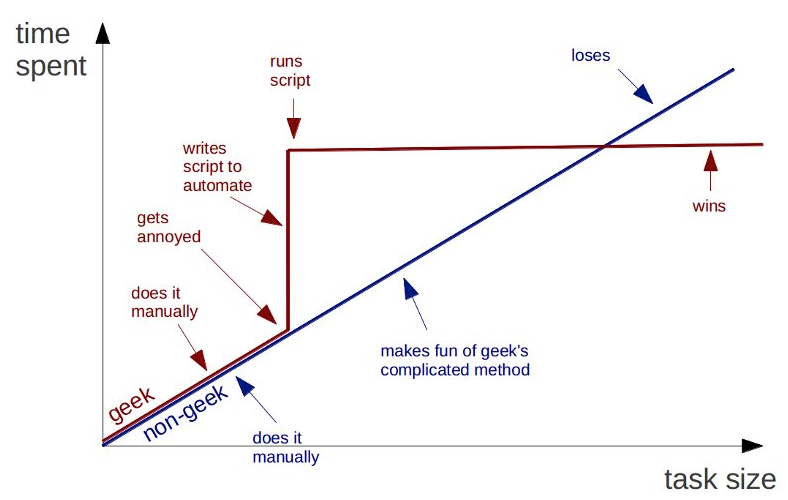
\includegraphics[scale=.5]{./files/figures/careful.png}
\caption{Recall we want to script to SAVE time}
\end{figure}

\begin{quote}
Image credit
\href{https://plus.google.com/102451193315916178828/posts/MGxauXypb1Y}{Bruno
Oliveira}
\end{quote}

    \begin{center}\rule{3in}{0.4pt}\end{center}

\subsection{Why Python is useful}\label{why-python-is-useful}

There are perhaps many reasons, here we list a few:

\begin{itemize}
\itemsep1pt\parskip0pt\parsep0pt
\item
  like other scripting languages, has an easier interface to learn
\item
  allow you to build your own work environment
\item
  scientific computing is more than crunching numbers
\item
  easier creation of GUIs, demos, and fancy HTML notebooks
\item
  create modern interfaces to old codes
\item
  allow you to explore, develop and test interactively
\item
  cleaner, shorter, easy to read, write, and maintain code
\end{itemize}

    \begin{center}\rule{3in}{0.4pt}\end{center}

\subsection{Is Python \textgreater{} MATLAB?}\label{is-python-matlab}

\subsubsection{Python == MATLAB}\label{python-matlab}

\begin{itemize}
\itemsep1pt\parskip0pt\parsep0pt
\item
  Simple and easy to use syntax (dynamic typing, array and linear
  algebra language)
\item
  Easy creation of interactive interfaces and GUIs
\item
  Merge simulation and visualization
\item
  Commercially supported (Continuum Analytics, Enthought)
\item
  Vibrant, enthusiastic academic communities for getting support and
  learning more
\item
  JIT support
\item
  Amazon EC2 support
\end{itemize}

\subsubsection{MATLAB \textgreater{} Python}\label{matlab-python}

\begin{itemize}
\itemsep1pt\parskip0pt\parsep0pt
\item
  Several MATLAB toolboxes offer capabilities unavailable to the Python
  community
\item
  Superior documentation
\item
  Commercially robust and reliable scientific computing tools
\end{itemize}

\subsubsection{Python \textgreater{} MATLAB}\label{python-matlab-1}

\begin{itemize}
\itemsep1pt\parskip0pt\parsep0pt
\item
  Python is free
\item
  Object-oriented programming is more convenient in Python
\item
  Extensive tools within and beyond scientific computing

  \begin{itemize}
  \itemsep1pt\parskip0pt\parsep0pt
  \item
    IPython notebook relies on a Python webserver as well as extensive
    asynchronous messaging support through PyZMQ
  \end{itemize}
\item
  Python runs on all modern Cray and IBM supercomputers (and anywhere C
  does)
\end{itemize}

    \begin{center}\rule{3in}{0.4pt}\end{center}

\section{Some Sample Applications}\label{some-sample-applications}

    \begin{center}\rule{3in}{0.4pt}\end{center}

\subsection{Teaching the finite element
method}\label{teaching-the-finite-element-method}

\subsubsection{Stiffness matrix
computation}\label{stiffness-matrix-computation}

\begin{figure}[htbp]
\centering
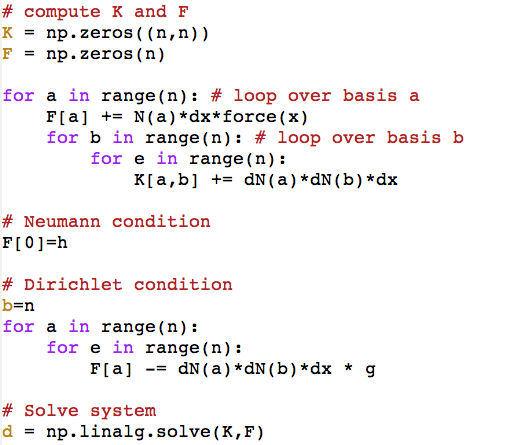
\includegraphics[scale=.5]{./files/figures/fem.png}
\caption{Stiffness matrix}
\end{figure}

    \begin{center}\rule{3in}{0.4pt}\end{center}

\subsection{Monitor program progress}\label{monitor-program-progress}

\subsubsection{Python parses a datafile and makes plots of current
progress}\label{python-parses-a-datafile-and-makes-plots-of-current-progress}

\begin{figure}[htbp]
\centering
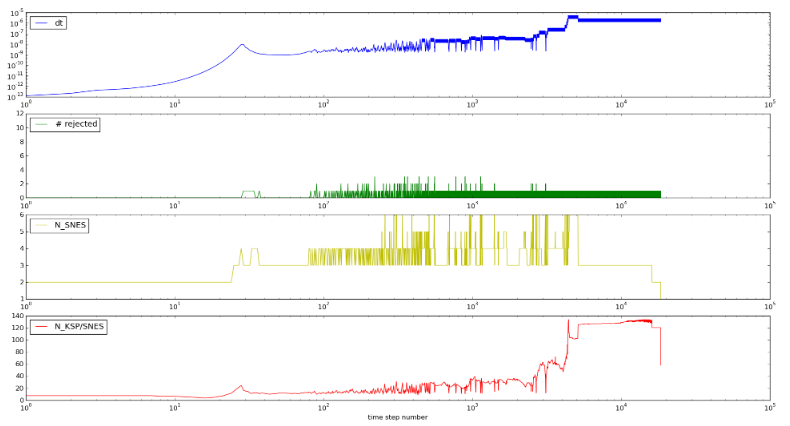
\includegraphics[scale=.5]{./files/figures/log.png}
\caption{Log}
\end{figure}

    \begin{center}\rule{3in}{0.4pt}\end{center}

\subsection{Problem prototypes}\label{problem-prototypes}

\subsubsection{Nonlinear, time dependent
problem}\label{nonlinear-time-dependent-problem}

\begin{figure}[htbp]
\centering
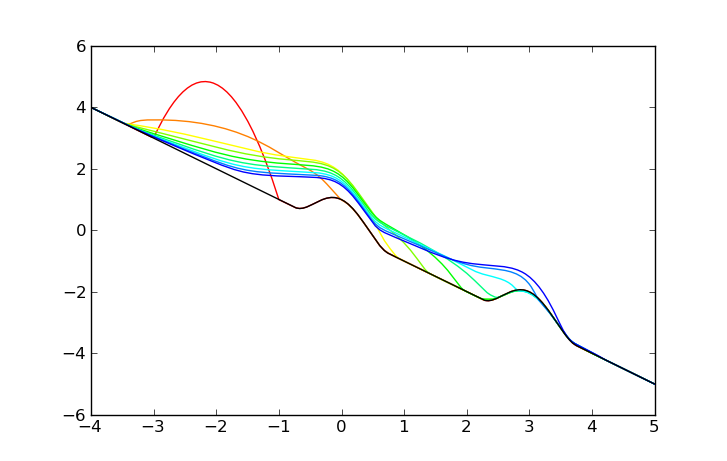
\includegraphics[scale=.5]{./files/figures/dsw.png}
\caption{NonLinear problem}
\end{figure}

    \begin{center}\rule{3in}{0.4pt}\end{center}

\subsection{Problem prototypes}\label{problem-prototypes}

\subsubsection{Method for fitting surface to
data}\label{method-for-fitting-surface-to-data}

\begin{figure}[htbp]
\centering
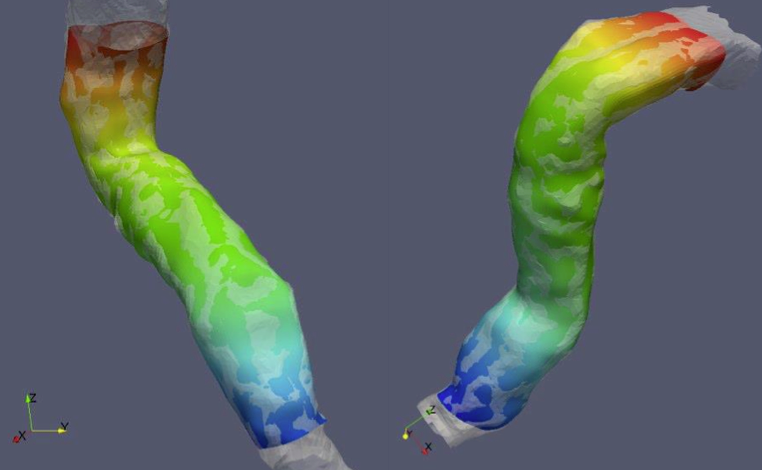
\includegraphics[scale=.5]{./files/figures/molt.png}
\caption{Prototypes}
\end{figure}

    \begin{center}\rule{3in}{0.4pt}\end{center}

\subsection{Structural program}\label{structural-program}

\subsubsection{Python manages floors and
columns}\label{python-manages-floors-and-columns}

\begin{figure}[htbp]
\centering
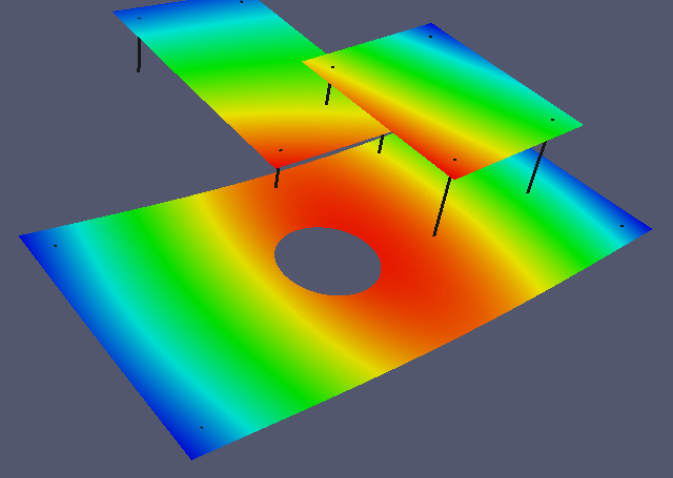
\includegraphics[scale=.5]{./files/figures/struct.png}
\caption{Structural program}
\end{figure}

    \begin{center}\rule{3in}{0.4pt}\end{center}

\subsection{Auto-generation of
results}\label{auto-generation-of-results}

\subsubsection{Python runs C code, post-processes the results, and
generates a LaTeX
table}\label{python-runs-c-code-post-processes-the-results-and-generates-a-latex-table}

\begin{figure}[htbp]
\centering
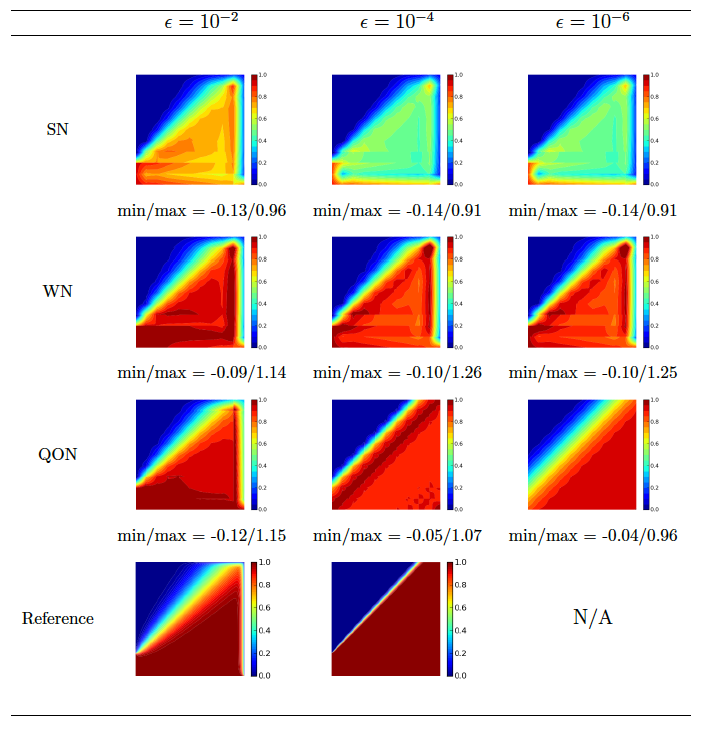
\includegraphics[scale=.5]{./files/figures/dpg.png}
\caption{Result Generation}
\end{figure}

    \begin{center}\rule{3in}{0.4pt}\end{center}

\section{A Tour of Python for Simple
Scripting}\label{a-tour-of-python-for-simple-scripting}

    \begin{center}\rule{3in}{0.4pt}\end{center}

\subsection{Script 1}\label{script-1}

    \begin{Verbatim}[commandchars=\\\{\}]
{\color{incolor}In [{\color{incolor}2}]:} \PY{c}{\PYZsh{}!/usr/bin/env python}
        \PY{k+kn}{import} \PY{n+nn}{math}
        \PY{n}{r} \PY{o}{=} \PY{n}{math}\PY{o}{.}\PY{n}{pi} \PY{o}{/} \PY{l+m+mf}{2.0}
        \PY{n}{s} \PY{o}{=} \PY{n}{math}\PY{o}{.}\PY{n}{sin}\PY{p}{(}\PY{n}{r}\PY{p}{)}
        \PY{k}{print} \PY{l+s}{\PYZdq{}}\PY{l+s}{Hello world, sin(}\PY{l+s+si}{\PYZpc{}f}\PY{l+s}{)=}\PY{l+s+si}{\PYZpc{}f}\PY{l+s}{\PYZdq{}} \PY{o}{\PYZpc{}} \PY{p}{(}\PY{n}{r}\PY{p}{,}\PY{n}{s}\PY{p}{)}
\end{Verbatim}

    \begin{Verbatim}[commandchars=\\\{\}]
Hello world, sin(1.570796)=1.000000
    \end{Verbatim}

    \begin{center}\rule{3in}{0.4pt}\end{center}

\subsection{Script 2}\label{script-2}

    \begin{Verbatim}[commandchars=\\\{\}]
{\color{incolor}In [{\color{incolor}5}]:} \PY{k+kn}{import} \PY{n+nn}{math}
        \PY{n}{infile} \PY{o}{=} \PY{l+s}{\PYZdq{}}\PY{l+s}{files/examples/data/numbers}\PY{l+s}{\PYZdq{}}
        \PY{n}{outfile} \PY{o}{=} \PY{l+s}{\PYZdq{}}\PY{l+s}{files/examples/data/f\PYZus{}numbers}\PY{l+s}{\PYZdq{}}
        
        \PY{n}{f} \PY{o}{=} \PY{n+nb}{open}\PY{p}{(}\PY{n}{infile}\PY{p}{,}\PY{l+s}{\PYZsq{}}\PY{l+s}{r}\PY{l+s}{\PYZsq{}}\PY{p}{)}
        \PY{n}{g} \PY{o}{=} \PY{n+nb}{open}\PY{p}{(}\PY{n}{outfile}\PY{p}{,}\PY{l+s}{\PYZsq{}}\PY{l+s}{w}\PY{l+s}{\PYZsq{}}\PY{p}{)}
        
        \PY{k}{def} \PY{n+nf}{func}\PY{p}{(}\PY{n}{y}\PY{p}{)}\PY{p}{:}
            \PY{k}{if} \PY{n}{y} \PY{o}{\PYZgt{}}\PY{o}{=} \PY{l+m+mf}{0.0}\PY{p}{:}
                \PY{k}{return} \PY{n}{y}\PY{o}{*}\PY{o}{*}\PY{l+m+mf}{5.0}\PY{o}{*}\PY{n}{math}\PY{o}{.}\PY{n}{exp}\PY{p}{(}\PY{o}{\PYZhy{}}\PY{n}{y}\PY{p}{)}
            \PY{k}{else}\PY{p}{:}
                \PY{k}{return} \PY{l+m+mf}{0.0}
            
        \PY{k}{for} \PY{n}{line} \PY{o+ow}{in} \PY{n}{f}\PY{p}{:}
            \PY{n}{line} \PY{o}{=} \PY{n}{line}\PY{o}{.}\PY{n}{split}\PY{p}{(}\PY{p}{)}
            \PY{n}{x} \PY{o}{=} \PY{n+nb}{float}\PY{p}{(}\PY{n}{line}\PY{p}{[}\PY{l+m+mi}{0}\PY{p}{]}\PY{p}{)}
            \PY{n}{y} \PY{o}{=} \PY{n+nb}{float}\PY{p}{(}\PY{n}{line}\PY{p}{[}\PY{l+m+mi}{1}\PY{p}{]}\PY{p}{)}
            \PY{n}{fy} \PY{o}{=} \PY{n}{func}\PY{p}{(}\PY{n}{y}\PY{p}{)}
            \PY{n}{g}\PY{o}{.}\PY{n}{write}\PY{p}{(}\PY{l+s}{\PYZdq{}}\PY{l+s+si}{\PYZpc{}g}\PY{l+s}{ }\PY{l+s+si}{\PYZpc{}12.5e}\PY{l+s+se}{\PYZbs{}n}\PY{l+s}{\PYZdq{}} \PY{o}{\PYZpc{}} \PY{p}{(}\PY{n}{x}\PY{p}{,}\PY{n}{fy}\PY{p}{)}\PY{p}{)}
            
        \PY{n}{f}\PY{o}{.}\PY{n}{close}\PY{p}{(}\PY{p}{)} 
        \PY{n}{g}\PY{o}{.}\PY{n}{close}\PY{p}{(}\PY{p}{)}
\end{Verbatim}

    \begin{center}\rule{3in}{0.4pt}\end{center}

\subsection{Script 3}\label{script-3}

    \begin{Verbatim}[commandchars=\\\{\}]
{\color{incolor}In [{\color{incolor}9}]:} \PY{k+kn}{import} \PY{n+nn}{sys}\PY{o}{,}\PY{n+nn}{os}
        \PY{n}{cmd} \PY{o}{=} \PY{l+s}{\PYZsq{}}\PY{l+s}{date}\PY{l+s}{\PYZsq{}}
        \PY{n}{output} \PY{o}{=} \PY{n}{os}\PY{o}{.}\PY{n}{popen}\PY{p}{(}\PY{n}{cmd}\PY{p}{)}
        \PY{n}{lines} \PY{o}{=} \PY{n}{output}\PY{o}{.}\PY{n}{readlines}\PY{p}{(}\PY{p}{)}
        \PY{n}{fail} \PY{o}{=} \PY{n}{output}\PY{o}{.}\PY{n}{close}\PY{p}{(}\PY{p}{)}
        \PY{k}{if} \PY{n}{fail}\PY{p}{:} \PY{k}{print} \PY{l+s}{\PYZsq{}}\PY{l+s}{You do not have the date command}\PY{l+s}{\PYZsq{}}\PY{p}{;} \PY{n}{sys}\PY{o}{.}\PY{n}{exit}\PY{p}{(}\PY{p}{)}
        \PY{k}{for} \PY{n}{line} \PY{o+ow}{in} \PY{n}{lines}\PY{p}{:}
            \PY{n}{line} \PY{o}{=} \PY{n}{line}\PY{o}{.}\PY{n}{split}\PY{p}{(}\PY{p}{)}
            \PY{k}{print} \PY{l+s}{\PYZdq{}}\PY{l+s}{The current time is }\PY{l+s+si}{\PYZpc{}s}\PY{l+s}{ on }\PY{l+s+si}{\PYZpc{}s}\PY{l+s}{ }\PY{l+s+si}{\PYZpc{}s}\PY{l+s}{, }\PY{l+s+si}{\PYZpc{}s}\PY{l+s}{\PYZdq{}} \PY{o}{\PYZpc{}} \PY{p}{(}\PY{n}{line}\PY{p}{[}\PY{l+m+mi}{3}\PY{p}{]}\PY{p}{,}\PY{n}{line}\PY{p}{[}\PY{l+m+mi}{2}\PY{p}{]}\PY{p}{,}\PY{n}{line}\PY{p}{[}\PY{l+m+mi}{1}\PY{p}{]}\PY{p}{,}\PY{n}{line}\PY{p}{[}\PY{o}{\PYZhy{}}\PY{l+m+mi}{1}\PY{p}{]}\PY{p}{)}
\end{Verbatim}

    \begin{Verbatim}[commandchars=\\\{\}]
The current time is 10:14:20 on 4 Sep, 2014
    \end{Verbatim}

    \begin{center}\rule{3in}{0.4pt}\end{center}

\subsection{Script 4}\label{script-4}

    \begin{center}\rule{3in}{0.4pt}\end{center}

\subsection{A bib-file (see
examples/data/python.bib)}\label{a-bib-file-see-examplesdatapython.bib}

\begin{verbatim}
@Book{Langtangen2011,
  author =    {Hans Petter Langtangen},
  title =     {A Primer on Scientific Programming with Python},
  publisher = {Springer},
  year =      {2011}
}
@Book{Langtangen2010,
  author =    {Hans Petter Langtangen},
  title =     {Python Scripting for Computational Science},
  publisher = {Springer},
  year =      {2010}
}
\end{verbatim}

    \begin{Verbatim}[commandchars=\\\{\}]
{\color{incolor}In [{\color{incolor}8}]:} \PY{k+kn}{import} \PY{n+nn}{re}
        \PY{n}{pattern1} \PY{o}{=} \PY{l+s}{\PYZdq{}}\PY{l+s}{@Book\PYZob{}(.*),}\PY{l+s}{\PYZdq{}}
        \PY{n}{pattern2} \PY{o}{=} \PY{l+s}{\PYZdq{}}\PY{l+s}{\PYZbs{}}\PY{l+s}{s+title}\PY{l+s}{\PYZbs{}}\PY{l+s}{s+=}\PY{l+s}{\PYZbs{}}\PY{l+s}{s+\PYZob{}(.*)\PYZcb{},}\PY{l+s}{\PYZdq{}}
        \PY{k}{for} \PY{n}{line} \PY{o+ow}{in} \PY{n+nb}{file}\PY{p}{(}\PY{l+s}{\PYZsq{}}\PY{l+s}{files/examples/data/python.bib}\PY{l+s}{\PYZsq{}}\PY{p}{)}\PY{p}{:}
            \PY{n}{match} \PY{o}{=} \PY{n}{re}\PY{o}{.}\PY{n}{search}\PY{p}{(}\PY{n}{pattern1}\PY{p}{,}\PY{n}{line}\PY{p}{)}
            \PY{k}{if} \PY{n}{match}\PY{p}{:} 
                \PY{k}{print} \PY{l+s}{\PYZdq{}}\PY{l+s}{Found a book with the tag }\PY{l+s}{\PYZsq{}}\PY{l+s+si}{\PYZpc{}s}\PY{l+s}{\PYZsq{}}\PY{l+s}{\PYZdq{}} \PY{o}{\PYZpc{}} \PY{n}{match}\PY{o}{.}\PY{n}{group}\PY{p}{(}\PY{l+m+mi}{1}\PY{p}{)}
            \PY{n}{match} \PY{o}{=} \PY{n}{re}\PY{o}{.}\PY{n}{search}\PY{p}{(}\PY{n}{pattern2}\PY{p}{,}\PY{n}{line}\PY{p}{)}
            \PY{k}{if} \PY{n}{match}\PY{p}{:}
                \PY{k}{print} \PY{l+s}{\PYZdq{}}\PY{l+s}{The title is }\PY{l+s}{\PYZsq{}}\PY{l+s+si}{\PYZpc{}s}\PY{l+s}{\PYZsq{}}\PY{l+s}{\PYZdq{}} \PY{o}{\PYZpc{}} \PY{n}{match}\PY{o}{.}\PY{n}{group}\PY{p}{(}\PY{l+m+mi}{1}\PY{p}{)}
\end{Verbatim}

    \begin{Verbatim}[commandchars=\\\{\}]
Found a book with the tag 'Langtangen2011'
The title is 'A Primer on Scientific Programming with Python'
Found a book with the tag 'Langtangen2010'
The title is 'Python Scripting for Computational Science'
    \end{Verbatim}

    \begin{center}\rule{3in}{0.4pt}\end{center}

\section{A Tour of Python for Scientific
Computing}\label{a-tour-of-python-for-scientific-computing}

    \begin{center}\rule{3in}{0.4pt}\end{center}

\subsection{Arrays}\label{arrays}

\textbf{Python} has built-in:

containers: lists (costless insertion and append), dictionaries (fast
lookup)\\high-level number objects: integers, floating point

\textbf{Numpy} is:

extension package to Python for multi-dimensional arrays\\closer to
hardware (efficiency)\\designed for scientific computation (convenience)

    \begin{Verbatim}[commandchars=\\\{\}]
{\color{incolor}In [{\color{incolor}11}]:} \PY{n}{a} \PY{o}{=} \PY{n}{np}\PY{o}{.}\PY{n}{array}\PY{p}{(}\PY{p}{[}\PY{l+m+mi}{0}\PY{p}{,}\PY{l+m+mi}{1}\PY{p}{,}\PY{l+m+mi}{2}\PY{p}{,}\PY{l+m+mi}{3}\PY{p}{,}\PY{l+m+mi}{4}\PY{p}{]}\PY{p}{)}
         \PY{n}{a}
\end{Verbatim}

            \begin{Verbatim}[commandchars=\\\{\}]
{\color{outcolor}Out[{\color{outcolor}11}]:} array([0, 1, 2, 3, 4])
\end{Verbatim}
        
    \begin{Verbatim}[commandchars=\\\{\}]
{\color{incolor}In [{\color{incolor}12}]:} \PY{k}{print} \PY{n}{a}\PY{o}{.}\PY{n}{ndim} \PY{c}{\PYZsh{} Dimensionality}
         \PY{k}{print} \PY{n}{a}\PY{o}{.}\PY{n}{shape} \PY{c}{\PYZsh{} Shape}
\end{Verbatim}

    \begin{Verbatim}[commandchars=\\\{\}]
1
(5,)
    \end{Verbatim}

    \begin{Verbatim}[commandchars=\\\{\}]
{\color{incolor}In [{\color{incolor}13}]:} \PY{n}{b} \PY{o}{=} \PY{n}{np}\PY{o}{.}\PY{n}{array}\PY{p}{(}\PY{p}{[}\PY{p}{[}\PY{l+m+mi}{0}\PY{p}{,} \PY{l+m+mi}{1}\PY{p}{,} \PY{l+m+mi}{2}\PY{p}{]}\PY{p}{,} \PY{p}{[}\PY{l+m+mi}{3}\PY{p}{,} \PY{l+m+mi}{4}\PY{p}{,} \PY{l+m+mi}{5}\PY{p}{]}\PY{p}{]}\PY{p}{)}
         \PY{k}{print} \PY{n}{b}
         \PY{k}{print} \PY{n}{b}\PY{o}{.}\PY{n}{ndim}
         \PY{k}{print} \PY{n}{b}\PY{o}{.}\PY{n}{shape}
\end{Verbatim}

    \begin{Verbatim}[commandchars=\\\{\}]
[[0 1 2]
 [3 4 5]]
2
(2, 3)
    \end{Verbatim}

    \begin{center}\rule{3in}{0.4pt}\end{center}

\subsection{Common Arrays}\label{common-arrays}

    \begin{Verbatim}[commandchars=\\\{\}]
{\color{incolor}In [{\color{incolor}14}]:} \PY{k}{print} \PY{n}{np}\PY{o}{.}\PY{n}{arange}\PY{p}{(}\PY{l+m+mi}{10}\PY{p}{)} \PY{c}{\PYZsh{} Like range [0, 1, ..., 9]}
         \PY{k}{print} \PY{n}{np}\PY{o}{.}\PY{n}{arange}\PY{p}{(}\PY{l+m+mi}{1}\PY{p}{,}\PY{l+m+mi}{9}\PY{p}{,} \PY{l+m+mi}{2}\PY{p}{)} \PY{c}{\PYZsh{} [1, 3, 5, 7]}
\end{Verbatim}

    \begin{Verbatim}[commandchars=\\\{\}]
[0 1 2 3 4 5 6 7 8 9]
[1 3 5 7]
    \end{Verbatim}

    \begin{Verbatim}[commandchars=\\\{\}]
{\color{incolor}In [{\color{incolor}15}]:} \PY{k}{print} \PY{n}{np}\PY{o}{.}\PY{n}{linspace}\PY{p}{(}\PY{l+m+mi}{0}\PY{p}{,} \PY{l+m+mi}{1}\PY{p}{,} \PY{l+m+mi}{6}\PY{p}{)} \PY{c}{\PYZsh{} A linear space of [0,1] with 6 pts}
         \PY{k}{print} \PY{n}{np}\PY{o}{.}\PY{n}{linspace}\PY{p}{(}\PY{l+m+mi}{0}\PY{p}{,} \PY{l+m+mi}{1}\PY{p}{,} \PY{l+m+mi}{6}\PY{p}{,} \PY{n}{endpoint}\PY{o}{=}\PY{n+nb+bp}{False}\PY{p}{)} \PY{c}{\PYZsh{} [0,1[}
\end{Verbatim}

    \begin{Verbatim}[commandchars=\\\{\}]
[ 0.   0.2  0.4  0.6  0.8  1. ]
[ 0.          0.16666667  0.33333333  0.5         0.66666667  0.83333333]
    \end{Verbatim}

    \begin{Verbatim}[commandchars=\\\{\}]
{\color{incolor}In [{\color{incolor}16}]:} \PY{k}{print} \PY{n}{np}\PY{o}{.}\PY{n}{ones}\PY{p}{(}\PY{p}{(}\PY{l+m+mi}{3}\PY{p}{,}\PY{l+m+mi}{3}\PY{p}{)}\PY{p}{)} \PY{c}{\PYZsh{} 3 X 3 2D array of 1\PYZsq{}s}
\end{Verbatim}

    \begin{Verbatim}[commandchars=\\\{\}]
[[ 1.  1.  1.]
 [ 1.  1.  1.]
 [ 1.  1.  1.]]
    \end{Verbatim}

    \begin{Verbatim}[commandchars=\\\{\}]
{\color{incolor}In [{\color{incolor}17}]:} \PY{k}{print} \PY{n}{np}\PY{o}{.}\PY{n}{eye}\PY{p}{(}\PY{l+m+mi}{3}\PY{p}{)}
\end{Verbatim}

    \begin{Verbatim}[commandchars=\\\{\}]
[[ 1.  0.  0.]
 [ 0.  1.  0.]
 [ 0.  0.  1.]]
    \end{Verbatim}

    \begin{Verbatim}[commandchars=\\\{\}]
{\color{incolor}In [{\color{incolor}18}]:} \PY{k}{print} \PY{n}{np}\PY{o}{.}\PY{n}{diag}\PY{p}{(}\PY{n}{arange}\PY{p}{(}\PY{l+m+mi}{4}\PY{p}{)}\PY{p}{)}
\end{Verbatim}

    \begin{Verbatim}[commandchars=\\\{\}]
[[0 0 0 0]
 [0 1 0 0]
 [0 0 2 0]
 [0 0 0 3]]
    \end{Verbatim}

    \begin{Verbatim}[commandchars=\\\{\}]
{\color{incolor}In [{\color{incolor}21}]:} \PY{k}{print} \PY{n}{np}\PY{o}{.}\PY{n}{random}\PY{o}{.}\PY{n}{rand}\PY{p}{(}\PY{l+m+mi}{4}\PY{p}{)} \PY{c}{\PYZsh{} Uniform distribution}
         \PY{k}{print} \PY{n}{np}\PY{o}{.}\PY{n}{random}\PY{o}{.}\PY{n}{randn}\PY{p}{(}\PY{l+m+mi}{4}\PY{p}{)} \PY{c}{\PYZsh{} Gaussian distribution}
\end{Verbatim}

    \begin{Verbatim}[commandchars=\\\{\}]
[ 0.9134486   0.7943014   0.40743464  0.8400922 ]
[-0.05662066 -0.99363921  0.35042966 -0.29096857]
    \end{Verbatim}

    \begin{Verbatim}[commandchars=\\\{\}]
{\color{incolor}In [{\color{incolor}27}]:} \PY{n}{hist}\PY{p}{(}\PY{n}{np}\PY{o}{.}\PY{n}{random}\PY{o}{.}\PY{n}{rand}\PY{p}{(}\PY{l+m+mi}{10000}\PY{p}{)}\PY{p}{,} \PY{n}{bins}\PY{o}{=}\PY{n}{np}\PY{o}{.}\PY{n}{linspace}\PY{p}{(}\PY{l+m+mi}{0}\PY{p}{,} \PY{l+m+mi}{1}\PY{p}{,} \PY{l+m+mi}{20}\PY{p}{,} \PY{n}{endpoint}\PY{o}{=}\PY{n+nb+bp}{False}\PY{p}{)}\PY{p}{)}\PY{p}{;}
\end{Verbatim}

    \begin{center}
    \adjustimage{max size={0.9\linewidth}{0.9\paperheight}}{01_Introducing_Python_files/01_Introducing_Python_44_0.png}
    \end{center}
    { \hspace*{\fill} \\}
    
    \begin{Verbatim}[commandchars=\\\{\}]
{\color{incolor}In [{\color{incolor}35}]:} \PY{n}{hist}\PY{p}{(}\PY{n}{np}\PY{o}{.}\PY{n}{random}\PY{o}{.}\PY{n}{randn}\PY{p}{(}\PY{l+m+mi}{50000}\PY{p}{)}\PY{p}{,} \PY{n}{bins}\PY{o}{=}\PY{n}{np}\PY{o}{.}\PY{n}{linspace}\PY{p}{(}\PY{o}{\PYZhy{}}\PY{l+m+mi}{5}\PY{p}{,} \PY{l+m+mi}{5}\PY{p}{,} \PY{l+m+mi}{100}\PY{p}{,} \PY{n}{endpoint}\PY{o}{=}\PY{n+nb+bp}{False}\PY{p}{)}\PY{p}{)}\PY{p}{;}
\end{Verbatim}

    \begin{center}
    \adjustimage{max size={0.9\linewidth}{0.9\paperheight}}{01_Introducing_Python_files/01_Introducing_Python_45_0.png}
    \end{center}
    { \hspace*{\fill} \\}
    
    \begin{center}\rule{3in}{0.4pt}\end{center}

\subsection{Other Numpy Features to be aware
of}\label{other-numpy-features-to-be-aware-of}

\begin{itemize}
\itemsep1pt\parskip0pt\parsep0pt
\item
  Reshaping
\end{itemize}

    \begin{Verbatim}[commandchars=\\\{\}]
{\color{incolor}In [{\color{incolor}36}]:} \PY{n}{arr} \PY{o}{=} \PY{n}{np}\PY{o}{.}\PY{n}{arange}\PY{p}{(}\PY{l+m+mi}{1000000}\PY{p}{)}
         \PY{n}{arr2} \PY{o}{=} \PY{n}{arr}\PY{o}{.}\PY{n}{reshape}\PY{p}{(}\PY{p}{(}\PY{l+m+mi}{10}\PY{p}{,}\PY{l+m+mi}{100000}\PY{p}{)}\PY{p}{)}
         \PY{k}{print}\PY{p}{(}\PY{n}{arr2}\PY{p}{)}
\end{Verbatim}

    \begin{Verbatim}[commandchars=\\\{\}]
[[     0      1      2 \ldots,  99997  99998  99999]
 [100000 100001 100002 \ldots, 199997 199998 199999]
 [200000 200001 200002 \ldots, 299997 299998 299999]
 \ldots, 
 [700000 700001 700002 \ldots, 799997 799998 799999]
 [800000 800001 800002 \ldots, 899997 899998 899999]
 [900000 900001 900002 \ldots, 999997 999998 999999]]
    \end{Verbatim}

    \begin{itemize}
\itemsep1pt\parskip0pt\parsep0pt
\item
  Memory Views
\end{itemize}

    \begin{Verbatim}[commandchars=\\\{\}]
{\color{incolor}In [{\color{incolor}37}]:} \PY{n}{arr2}\PY{o}{.}\PY{n}{view}\PY{err}{?}
\end{Verbatim}

    \begin{itemize}
\itemsep1pt\parskip0pt\parsep0pt
\item
  Index Slicing
\end{itemize}

    \begin{Verbatim}[commandchars=\\\{\}]
{\color{incolor}In [{\color{incolor}38}]:} \PY{n}{x} \PY{o}{=} \PY{n}{np}\PY{o}{.}\PY{n}{arange}\PY{p}{(}\PY{l+m+mi}{0}\PY{p}{,} \PY{l+m+mi}{20}\PY{p}{,} \PY{l+m+mi}{2}\PY{p}{)}\PY{p}{;} \PY{n}{y} \PY{o}{=} \PY{n}{x}\PY{o}{*}\PY{o}{*}\PY{l+m+mi}{2}
         \PY{p}{(}\PY{p}{(}\PY{n}{y}\PY{p}{[}\PY{l+m+mi}{1}\PY{p}{:}\PY{p}{]} \PY{o}{\PYZhy{}} \PY{n}{y}\PY{p}{[}\PY{p}{:}\PY{o}{\PYZhy{}}\PY{l+m+mi}{1}\PY{p}{]}\PY{p}{)} \PY{o}{/} \PY{p}{(}\PY{n}{x}\PY{p}{[}\PY{l+m+mi}{1}\PY{p}{:}\PY{p}{]} \PY{o}{\PYZhy{}} \PY{n}{x}\PY{p}{[}\PY{p}{:}\PY{o}{\PYZhy{}}\PY{l+m+mi}{1}\PY{p}{]}\PY{p}{)}\PY{p}{)} \PY{c}{\PYZsh{} dy/dx}
\end{Verbatim}

            \begin{Verbatim}[commandchars=\\\{\}]
{\color{outcolor}Out[{\color{outcolor}38}]:} array([ 2,  6, 10, 14, 18, 22, 26, 30, 34])
\end{Verbatim}
        
    \begin{itemize}
\itemsep1pt\parskip0pt\parsep0pt
\item
  Fancy Indexing
\end{itemize}

    \begin{Verbatim}[commandchars=\\\{\}]
{\color{incolor}In [{\color{incolor}39}]:} \PY{n}{evens} \PY{o}{=} \PY{n}{arr}\PY{p}{[}\PY{n}{arr}\PY{o}{\PYZpc{}}\PY{k}{2} \PY{o}{==} \PY{l+m+mi}{0}\PY{p}{]}
         \PY{k}{print}\PY{p}{(}\PY{n}{evens}\PY{p}{)}
\end{Verbatim}

    \begin{Verbatim}[commandchars=\\\{\}]
[     0      2      4 \ldots, 999994 999996 999998]
    \end{Verbatim}

    \begin{center}\rule{3in}{0.4pt}\end{center}

\subsection{LinAlg, FFTs, and Random
numbers}\label{linalg-ffts-and-random-numbers}

    \begin{Verbatim}[commandchars=\\\{\}]
{\color{incolor}In [{\color{incolor}40}]:} \PY{n}{np}\PY{o}{.}\PY{n}{dot}\PY{p}{(}\PY{n}{arange}\PY{p}{(}\PY{l+m+mi}{10}\PY{p}{)}\PY{p}{,} \PY{n}{arange}\PY{p}{(}\PY{l+m+mi}{10}\PY{p}{)}\PY{p}{)}
\end{Verbatim}

            \begin{Verbatim}[commandchars=\\\{\}]
{\color{outcolor}Out[{\color{outcolor}40}]:} 285
\end{Verbatim}
        
    \begin{Verbatim}[commandchars=\\\{\}]
{\color{incolor}In [{\color{incolor}41}]:} \PY{n}{np}\PY{o}{.}\PY{n}{dot}\PY{p}{(}\PY{n}{arange}\PY{p}{(}\PY{l+m+mi}{9}\PY{p}{)}\PY{o}{.}\PY{n}{reshape}\PY{p}{(}\PY{l+m+mi}{3}\PY{p}{,}\PY{l+m+mi}{3}\PY{p}{)}\PY{p}{,}
             \PY{n}{arange}\PY{p}{(}\PY{l+m+mi}{9}\PY{p}{)}\PY{o}{.}\PY{n}{reshape}\PY{p}{(}\PY{l+m+mi}{3}\PY{p}{,}\PY{l+m+mi}{3}\PY{p}{)}\PY{p}{)}
\end{Verbatim}

            \begin{Verbatim}[commandchars=\\\{\}]
{\color{outcolor}Out[{\color{outcolor}41}]:} array([[ 15,  18,  21],
                [ 42,  54,  66],
                [ 69,  90, 111]])
\end{Verbatim}
        
    \begin{Verbatim}[commandchars=\\\{\}]
{\color{incolor}In [{\color{incolor}42}]:} \PY{n}{np}\PY{o}{.}\PY{n}{fft}\PY{err}{?}
\end{Verbatim}

    \begin{Verbatim}[commandchars=\\\{\}]
{\color{incolor}In [{\color{incolor}43}]:} \PY{n}{np}\PY{o}{.}\PY{n}{linalg}\PY{err}{?}
\end{Verbatim}

    \begin{Verbatim}[commandchars=\\\{\}]
{\color{incolor}In [{\color{incolor}23}]:} \PY{n}{np}\PY{o}{.}\PY{n}{random}\PY{err}{?}
\end{Verbatim}

    \begin{center}\rule{3in}{0.4pt}\end{center}

\subsection{Quick Visualization /
MatPlotLib}\label{quick-visualization-matplotlib}

How quickly can we plot 10K numbers?

    \begin{Verbatim}[commandchars=\\\{\}]
{\color{incolor}In [{\color{incolor}44}]:} \PY{n}{\PYZus{}} \PY{o}{=} \PY{n}{hist}\PY{p}{(}\PY{n}{random}\PY{o}{.}\PY{n}{randn}\PY{p}{(}\PY{l+m+mi}{100000}\PY{p}{)}\PY{p}{,} \PY{l+m+mi}{100}\PY{p}{)}
\end{Verbatim}

    \begin{center}
    \adjustimage{max size={0.9\linewidth}{0.9\paperheight}}{01_Introducing_Python_files/01_Introducing_Python_61_0.png}
    \end{center}
    { \hspace*{\fill} \\}
    
    \begin{center}\rule{3in}{0.4pt}\end{center}

\subsection{Basic Plotting}\label{basic-plotting}

    \begin{Verbatim}[commandchars=\\\{\}]
{\color{incolor}In [{\color{incolor}45}]:} \PY{n}{\PYZus{}} \PY{o}{=} \PY{n}{plot}\PY{p}{(}\PY{n+nb}{range}\PY{p}{(}\PY{l+m+mi}{100}\PY{p}{)}\PY{p}{)}
         \PY{n}{\PYZus{}} \PY{o}{=} \PY{n}{xlabel}\PY{p}{(}\PY{l+s}{\PYZdq{}}\PY{l+s}{measured}\PY{l+s}{\PYZdq{}}\PY{p}{)}
         \PY{n}{\PYZus{}} \PY{o}{=} \PY{n}{ylabel}\PY{p}{(}\PY{l+s}{\PYZdq{}}\PY{l+s}{calculated}\PY{l+s}{\PYZdq{}}\PY{p}{)}
         \PY{n}{grid}\PY{p}{(}\PY{n+nb+bp}{True}\PY{p}{)}
\end{Verbatim}

    \begin{center}
    \adjustimage{max size={0.9\linewidth}{0.9\paperheight}}{01_Introducing_Python_files/01_Introducing_Python_63_0.png}
    \end{center}
    { \hspace*{\fill} \\}
    
    \begin{Verbatim}[commandchars=\\\{\}]
{\color{incolor}In [{\color{incolor}46}]:} \PY{n}{x} \PY{o}{=} \PY{p}{[}\PY{n}{val}\PY{o}{*}\PY{o}{.}\PY{l+m+mo}{01} \PY{k}{for} \PY{n}{val} \PY{o+ow}{in} \PY{n+nb}{range}\PY{p}{(}\PY{l+m+mi}{100}\PY{p}{)}\PY{p}{]}  \PY{c}{\PYZsh{} [0, .01, .02, ..., .98, .99]}
         \PY{n}{linear} \PY{o}{=} \PY{p}{[}\PY{n}{val} \PY{k}{for} \PY{n}{val} \PY{o+ow}{in} \PY{n}{x}\PY{p}{]} 
         \PY{n}{square} \PY{o}{=} \PY{p}{[}\PY{n}{val}\PY{o}{*}\PY{o}{*}\PY{l+m+mi}{2} \PY{k}{for} \PY{n}{val} \PY{o+ow}{in} \PY{n}{x}\PY{p}{]}
         \PY{n}{\PYZus{}} \PY{o}{=} \PY{n}{plot}\PY{p}{(}\PY{n}{x}\PY{p}{,} \PY{n}{linear}\PY{p}{,} \PY{n}{x}\PY{p}{,} \PY{n}{square}\PY{p}{)}
\end{Verbatim}

    \begin{center}
    \adjustimage{max size={0.9\linewidth}{0.9\paperheight}}{01_Introducing_Python_files/01_Introducing_Python_64_0.png}
    \end{center}
    { \hspace*{\fill} \\}
    
    \begin{Verbatim}[commandchars=\\\{\}]
{\color{incolor}In [{\color{incolor}47}]:} \PY{n}{num\PYZus{}vals} \PY{o}{=} \PY{l+m+mi}{10}
         \PY{n}{x} \PY{o}{=} \PY{p}{[}\PY{n+nb}{float}\PY{p}{(}\PY{n}{val}\PY{p}{)}\PY{o}{/}\PY{n}{num\PYZus{}vals} \PY{k}{for} \PY{n}{val} \PY{o+ow}{in} \PY{n+nb}{range}\PY{p}{(}\PY{n}{num\PYZus{}vals}\PY{p}{)}\PY{p}{]}  \PY{c}{\PYZsh{} [0, .01, .02, ..., .98, .99]}
         \PY{n}{linear} \PY{o}{=} \PY{p}{[}\PY{n}{val} \PY{k}{for} \PY{n}{val} \PY{o+ow}{in} \PY{n}{x}\PY{p}{]} 
         \PY{n}{square} \PY{o}{=} \PY{p}{[}\PY{n}{val}\PY{o}{*}\PY{o}{*}\PY{l+m+mi}{2} \PY{k}{for} \PY{n}{val} \PY{o+ow}{in} \PY{n}{x}\PY{p}{]}
         \PY{n}{\PYZus{}}\PY{o}{=} \PY{n}{plot}\PY{p}{(}\PY{n}{x}\PY{p}{,} \PY{n}{linear}\PY{p}{,} \PY{l+s}{\PYZsq{}}\PY{l+s}{g:+}\PY{l+s}{\PYZsq{}}\PY{p}{,} \PY{n}{x}\PY{p}{,} \PY{n}{square}\PY{p}{,} \PY{l+s}{\PYZsq{}}\PY{l+s}{r\PYZhy{}\PYZhy{}o}\PY{l+s}{\PYZsq{}}\PY{p}{)}
\end{Verbatim}

    \begin{center}
    \adjustimage{max size={0.9\linewidth}{0.9\paperheight}}{01_Introducing_Python_files/01_Introducing_Python_65_0.png}
    \end{center}
    { \hspace*{\fill} \\}
    
    \begin{Verbatim}[commandchars=\\\{\}]
{\color{incolor}In [{\color{incolor}53}]:} \PY{n}{num\PYZus{}vals} \PY{o}{=} \PY{l+m+mi}{10}
         \PY{n}{x} \PY{o}{=} \PY{p}{[}\PY{n+nb}{float}\PY{p}{(}\PY{n}{val}\PY{p}{)}\PY{o}{/}\PY{n}{num\PYZus{}vals} \PY{k}{for} \PY{n}{val} \PY{o+ow}{in} \PY{n+nb}{range}\PY{p}{(}\PY{n}{num\PYZus{}vals}\PY{p}{)}\PY{p}{]}  \PY{c}{\PYZsh{} [0, .01, .02, ..., .98, .99]}
         \PY{n}{linear} \PY{o}{=} \PY{p}{[}\PY{n}{val} \PY{k}{for} \PY{n}{val} \PY{o+ow}{in} \PY{n}{x}\PY{p}{]} 
         \PY{n}{square} \PY{o}{=} \PY{p}{[}\PY{n}{val}\PY{o}{*}\PY{o}{*}\PY{l+m+mi}{2} \PY{k}{for} \PY{n}{val} \PY{o+ow}{in} \PY{n}{x}\PY{p}{]}
         \PY{n}{\PYZus{}} \PY{o}{=} \PY{n}{plot}\PY{p}{(}\PY{n}{x}\PY{p}{,} \PY{n}{linear}\PY{p}{,} \PY{l+s}{\PYZsq{}}\PY{l+s}{g:+}\PY{l+s}{\PYZsq{}}\PY{p}{,} \PY{n}{x}\PY{p}{,} \PY{n}{square}\PY{p}{,} \PY{l+s}{\PYZsq{}}\PY{l+s}{r\PYZhy{}\PYZhy{}o}\PY{l+s}{\PYZsq{}}\PY{p}{)}
         \PY{n}{\PYZus{}} \PY{o}{=} \PY{n}{legend}\PY{p}{(}\PY{p}{(}\PY{l+s}{\PYZsq{}}\PY{l+s}{linear}\PY{l+s}{\PYZsq{}}\PY{p}{,} \PY{l+s}{\PYZsq{}}\PY{l+s}{square}\PY{l+s}{\PYZsq{}}\PY{p}{)}\PY{p}{,} \PY{n}{loc}\PY{o}{=}\PY{l+s}{\PYZsq{}}\PY{l+s}{upper left}\PY{l+s}{\PYZsq{}}\PY{p}{)}
\end{Verbatim}

    \begin{center}
    \adjustimage{max size={0.9\linewidth}{0.9\paperheight}}{01_Introducing_Python_files/01_Introducing_Python_66_0.png}
    \end{center}
    { \hspace*{\fill} \\}
    
    \begin{Verbatim}[commandchars=\\\{\}]
{\color{incolor}In [{\color{incolor}54}]:} \PY{n}{\PYZus{}} \PY{o}{=} \PY{n}{plot}\PY{p}{(}\PY{n}{linear}\PY{p}{)}
         \PY{n}{\PYZus{}} \PY{o}{=} \PY{n}{axes}\PY{p}{(}\PY{p}{[}\PY{l+m+mf}{0.2}\PY{p}{,} \PY{l+m+mf}{0.5}\PY{p}{,} \PY{l+m+mf}{0.25}\PY{p}{,} \PY{l+m+mf}{0.25}\PY{p}{]}\PY{p}{)}
         \PY{n}{\PYZus{}} \PY{o}{=} \PY{n}{plot}\PY{p}{(}\PY{n}{square}\PY{p}{)}
\end{Verbatim}

    \begin{center}
    \adjustimage{max size={0.9\linewidth}{0.9\paperheight}}{01_Introducing_Python_files/01_Introducing_Python_67_0.png}
    \end{center}
    { \hspace*{\fill} \\}
    
    \begin{longtable}[c]{@{}l@{}}
\toprule\addlinespace
SciPy: Collection of High-Level Tools
\\\addlinespace
\bottomrule
\end{longtable}

\begin{itemize}
\itemsep1pt\parskip0pt\parsep0pt
\item
  mathematical algorithms and convenience functions built on the Numpy,
\item
  organized into subpackages covering different scientific computing
  domains,
\item
  a data-processing and system-prototyping environment rivaling sytems
  such as MATLAB, IDL, Octave, R-Lab, and SciLab
\end{itemize}

    \begin{longtable}[c]{@{}l@{}}
\toprule\addlinespace
SciPy: Collection of High-Level Tools
\\\addlinespace
\bottomrule
\end{longtable}

\begin{itemize}
\itemsep1pt\parskip0pt\parsep0pt
\item
  File IO (scipy.io)
\item
  Special functions (scipy.special)
\item
  Integration (scipy.integrate)
\item
  Optimization (scipy.optimize)
\item
  Interpolation (scipy.interpolate)
\item
  Fourier Transforms (scipy.fftpack)
\item
  Signal Processing (scipy.signal)
\item
  Linear Algebra (scipy.linalg)
\item
  Sparse Eigenvalue Problems with ARPACK
\item
  Statistics (scipy.stats)
\item
  Multi-dimensional image processing (scipy.ndimage)
\item
  Weave (scipy.weave)
\end{itemize}

    \begin{longtable}[c]{@{}l@{}}
\toprule\addlinespace
scipy.io
\\\addlinespace
\bottomrule
\end{longtable}

    \begin{Verbatim}[commandchars=\\\{\}]
{\color{incolor}In [{\color{incolor}55}]:} \PY{k+kn}{import} \PY{n+nn}{scipy}
         \PY{k+kn}{from} \PY{n+nn}{scipy} \PY{k+kn}{import} \PY{n}{io} \PY{k}{as} \PY{n}{spio}
         \PY{n}{a} \PY{o}{=} \PY{n}{np}\PY{o}{.}\PY{n}{ones}\PY{p}{(}\PY{p}{(}\PY{l+m+mi}{3}\PY{p}{,} \PY{l+m+mi}{3}\PY{p}{)}\PY{p}{)}
         \PY{n}{spio}\PY{o}{.}\PY{n}{savemat}\PY{p}{(}\PY{l+s}{\PYZsq{}}\PY{l+s}{file.mat}\PY{l+s}{\PYZsq{}}\PY{p}{,} \PY{p}{\PYZob{}}\PY{l+s}{\PYZsq{}}\PY{l+s}{a}\PY{l+s}{\PYZsq{}}\PY{p}{:} \PY{n}{a}\PY{p}{\PYZcb{}}\PY{p}{)} \PY{c}{\PYZsh{} savemat expects a dictionary}
         \PY{n}{data} \PY{o}{=} \PY{n}{spio}\PY{o}{.}\PY{n}{loadmat}\PY{p}{(}\PY{l+s}{\PYZsq{}}\PY{l+s}{file.mat}\PY{l+s}{\PYZsq{}}\PY{p}{,} \PY{n}{struct\PYZus{}as\PYZus{}record}\PY{o}{=}\PY{n+nb+bp}{True}\PY{p}{)}
         \PY{n}{data}\PY{p}{[}\PY{l+s}{\PYZsq{}}\PY{l+s}{a}\PY{l+s}{\PYZsq{}}\PY{p}{]}
\end{Verbatim}

    \begin{Verbatim}[commandchars=\\\{\}]
/Users/knepley/MacSoftware/lib/python2.7/site-packages/scipy/io/matlab/mio.py:267: FutureWarning: Using oned\_as default value ('column') This will change to 'row' in future versions
  oned\_as=oned\_as)
    \end{Verbatim}

            \begin{Verbatim}[commandchars=\\\{\}]
{\color{outcolor}Out[{\color{outcolor}55}]:} array([[ 1.,  1.,  1.],
                [ 1.,  1.,  1.],
                [ 1.,  1.,  1.]])
\end{Verbatim}
        
    Also see:

\begin{itemize}
\itemsep1pt\parskip0pt\parsep0pt
\item
  Images
\item
  IDL Files
\item
  Matrix Market Files
\item
  Wav files
\end{itemize}

    \begin{longtable}[c]{@{}l@{}}
\toprule\addlinespace
scipy.special
\\\addlinespace
\bottomrule
\end{longtable}

\begin{itemize}
\itemsep1pt\parskip0pt\parsep0pt
\item
  Bessel function, such as scipy.special.jn() (nth integer order Bessel
  function)
\item
  Elliptic function (scipy.special.ellipj() for the Jacobian elliptic
  function, \ldots{})
\item
  Gamma function: scipy.special.gamma(), also note
  scipy.special.gammaln() which will give the log of Gamma to a higher
  numerical precision.
\item
  Erf, the area under a Gaussian curve: scipy.special.erf()
\end{itemize}

    \begin{Verbatim}[commandchars=\\\{\}]
{\color{incolor}In [{\color{incolor}56}]:} \PY{k+kn}{from} \PY{n+nn}{scipy.special} \PY{k+kn}{import} \PY{n}{jn}
         \PY{n}{x} \PY{o}{=} \PY{n}{np}\PY{o}{.}\PY{n}{linspace}\PY{p}{(}\PY{l+m+mi}{0}\PY{p}{,} \PY{l+m+mi}{1}\PY{p}{,} \PY{l+m+mi}{10}\PY{p}{)}
         \PY{k}{print} \PY{p}{[}\PY{n}{jn}\PY{p}{(}\PY{n}{val}\PY{p}{,} \PY{l+m+mf}{1.0}\PY{p}{)} \PY{k}{for} \PY{n}{val} \PY{o+ow}{in} \PY{n}{x}\PY{p}{]}
\end{Verbatim}

    \begin{Verbatim}[commandchars=\\\{\}]
[0.76519768655796649, 0.77042135015704238, 0.75775886140714455, 0.73087640216944849, 
 0.69324418101264496, 0.64801456180958794, 0.59794997367362868, 0.54539073261127002,
 0.49225331977915776, 0.44005058574493355]
    \end{Verbatim}

    \begin{Verbatim}[commandchars=\\\{\}]
{\color{incolor}In [{\color{incolor}57}]:} \PY{k+kn}{from} \PY{n+nn}{scipy} \PY{k+kn}{import} \PY{o}{*}
         \PY{k+kn}{from} \PY{n+nn}{scipy.special} \PY{k+kn}{import} \PY{n}{jn}\PY{p}{,} \PY{n}{jn\PYZus{}zeros}
         \PY{k}{def} \PY{n+nf}{drumhead\PYZus{}height}\PY{p}{(}\PY{n}{n}\PY{p}{,} \PY{n}{k}\PY{p}{,} \PY{n}{distance}\PY{p}{,} \PY{n}{angle}\PY{p}{,} \PY{n}{t}\PY{p}{)}\PY{p}{:}
             \PY{n}{nth\PYZus{}zero} \PY{o}{=} \PY{n}{jn\PYZus{}zeros}\PY{p}{(}\PY{n}{n}\PY{p}{,} \PY{n}{k}\PY{p}{)}
             \PY{k}{return} \PY{n}{cos}\PY{p}{(}\PY{n}{t}\PY{p}{)}\PY{o}{*}\PY{n}{cos}\PY{p}{(}\PY{n}{n}\PY{o}{*}\PY{n}{angle}\PY{p}{)}\PY{o}{*}\PY{n}{jn}\PY{p}{(}\PY{n}{n}\PY{p}{,} \PY{n}{distance}\PY{o}{*}\PY{n}{nth\PYZus{}zero}\PY{p}{)}
         \PY{n}{theta} \PY{o}{=} \PY{n}{r\PYZus{}}\PY{p}{[}\PY{l+m+mi}{0}\PY{p}{:}\PY{l+m+mi}{2}\PY{o}{*}\PY{n}{pi}\PY{p}{:}\PY{l+m+mi}{50j}\PY{p}{]}
         \PY{n}{radius} \PY{o}{=} \PY{n}{r\PYZus{}}\PY{p}{[}\PY{l+m+mi}{0}\PY{p}{:}\PY{l+m+mi}{1}\PY{p}{:}\PY{l+m+mi}{50j}\PY{p}{]}
         \PY{n}{x} \PY{o}{=} \PY{n}{array}\PY{p}{(}\PY{p}{[}\PY{n}{r}\PY{o}{*}\PY{n}{cos}\PY{p}{(}\PY{n}{theta}\PY{p}{)} \PY{k}{for} \PY{n}{r} \PY{o+ow}{in} \PY{n}{radius}\PY{p}{]}\PY{p}{)}
         \PY{n}{y} \PY{o}{=} \PY{n}{array}\PY{p}{(}\PY{p}{[}\PY{n}{r}\PY{o}{*}\PY{n}{sin}\PY{p}{(}\PY{n}{theta}\PY{p}{)} \PY{k}{for} \PY{n}{r} \PY{o+ow}{in} \PY{n}{radius}\PY{p}{]}\PY{p}{)}
         \PY{n}{z} \PY{o}{=} \PY{n}{array}\PY{p}{(}\PY{p}{[}\PY{n}{drumhead\PYZus{}height}\PY{p}{(}\PY{l+m+mi}{1}\PY{p}{,} \PY{l+m+mi}{1}\PY{p}{,} \PY{n}{r}\PY{p}{,} \PY{n}{theta}\PY{p}{,} \PY{l+m+mf}{0.5}\PY{p}{)} \PY{k}{for} \PY{n}{r} \PY{o+ow}{in} \PY{n}{radius}\PY{p}{]}\PY{p}{)}
\end{Verbatim}

    \begin{Verbatim}[commandchars=\\\{\}]
{\color{incolor}In [{\color{incolor}58}]:} \PY{k+kn}{from} \PY{n+nn}{mpl\PYZus{}toolkits.mplot3d} \PY{k+kn}{import} \PY{n}{Axes3D}
         \PY{k+kn}{from} \PY{n+nn}{matplotlib} \PY{k+kn}{import} \PY{n}{cm}
         \PY{n}{fig} \PY{o}{=} \PY{n}{pylab}\PY{o}{.}\PY{n}{figure}\PY{p}{(}\PY{p}{)}
         \PY{n}{ax} \PY{o}{=} \PY{n}{Axes3D}\PY{p}{(}\PY{n}{fig}\PY{p}{)}
         \PY{n}{ax}\PY{o}{.}\PY{n}{plot\PYZus{}surface}\PY{p}{(}\PY{n}{x}\PY{p}{,} \PY{n}{y}\PY{p}{,} \PY{n}{z}\PY{p}{,} \PY{n}{rstride}\PY{o}{=}\PY{l+m+mi}{1}\PY{p}{,} \PY{n}{cstride}\PY{o}{=}\PY{l+m+mi}{1}\PY{p}{,} \PY{n}{cmap}\PY{o}{=}\PY{n}{cm}\PY{o}{.}\PY{n}{jet}\PY{p}{)}
         \PY{n}{\PYZus{}} \PY{o}{=} \PY{n}{ax}\PY{o}{.}\PY{n}{set\PYZus{}xlabel}\PY{p}{(}\PY{l+s}{\PYZsq{}}\PY{l+s}{X}\PY{l+s}{\PYZsq{}}\PY{p}{)}
         \PY{n}{\PYZus{}} \PY{o}{=} \PY{n}{ax}\PY{o}{.}\PY{n}{set\PYZus{}ylabel}\PY{p}{(}\PY{l+s}{\PYZsq{}}\PY{l+s}{Y}\PY{l+s}{\PYZsq{}}\PY{p}{)}
         \PY{n}{\PYZus{}} \PY{o}{=} \PY{n}{ax}\PY{o}{.}\PY{n}{set\PYZus{}zlabel}\PY{p}{(}\PY{l+s}{\PYZsq{}}\PY{l+s}{Z}\PY{l+s}{\PYZsq{}}\PY{p}{)}
\end{Verbatim}

    \begin{center}
    \adjustimage{max size={0.9\linewidth}{0.9\paperheight}}{01_Introducing_Python_files/01_Introducing_Python_76_0.png}
    \end{center}
    { \hspace*{\fill} \\}
    
    \begin{longtable}[c]{@{}l@{}}
\toprule\addlinespace
scipy.linalg
\\\addlinespace
\bottomrule
\end{longtable}

\begin{itemize}
\itemsep1pt\parskip0pt\parsep0pt
\item
  Matrix class (all routines still work with 2D NumPy arrays)
\item
  Basic Linear Algebra
\item
  Decompositions
\item
  Matrix Functions
\item
  Special matrices
\end{itemize}

    \begin{Verbatim}[commandchars=\\\{\}]
{\color{incolor}In [{\color{incolor}59}]:} \PY{n}{A} \PY{o}{=} \PY{n}{sp}\PY{o}{.}\PY{n}{mat}\PY{p}{(}\PY{l+s}{\PYZsq{}}\PY{l+s}{[1 3 5; 2 5 1; 2 3 8]}\PY{l+s}{\PYZsq{}}\PY{p}{)}
         \PY{n}{A}
\end{Verbatim}

            \begin{Verbatim}[commandchars=\\\{\}]
{\color{outcolor}Out[{\color{outcolor}59}]:} matrix([[1, 3, 5],
                 [2, 5, 1],
                 [2, 3, 8]])
\end{Verbatim}
        
    \begin{Verbatim}[commandchars=\\\{\}]
{\color{incolor}In [{\color{incolor}60}]:} \PY{n}{A}\PY{o}{.}\PY{n}{I}
\end{Verbatim}

            \begin{Verbatim}[commandchars=\\\{\}]
{\color{outcolor}Out[{\color{outcolor}60}]:} matrix([[-1.48,  0.36,  0.88],
                 [ 0.56,  0.08, -0.36],
                 [ 0.16, -0.12,  0.04]])
\end{Verbatim}
        
    \begin{Verbatim}[commandchars=\\\{\}]
{\color{incolor}In [{\color{incolor}61}]:} \PY{k+kn}{from} \PY{n+nn}{scipy} \PY{k+kn}{import} \PY{n}{linalg}
         \PY{n}{linalg}\PY{o}{.}\PY{n}{inv}\PY{p}{(}\PY{n}{A}\PY{p}{)}
\end{Verbatim}

            \begin{Verbatim}[commandchars=\\\{\}]
{\color{outcolor}Out[{\color{outcolor}61}]:} array([[-1.48,  0.36,  0.88],
                [ 0.56,  0.08, -0.36],
                [ 0.16, -0.12,  0.04]])
\end{Verbatim}
        
    \begin{Verbatim}[commandchars=\\\{\}]
{\color{incolor}In [{\color{incolor}62}]:} \PY{n}{linalg}\PY{o}{.}\PY{n}{svd}\PY{p}{(}\PY{n}{A}\PY{p}{)}
\end{Verbatim}

            \begin{Verbatim}[commandchars=\\\{\}]
{\color{outcolor}Out[{\color{outcolor}62}]:} (array([[-0.52956045,  0.04298197, -0.84718255],
                 [-0.34647857, -0.92256717,  0.16977167],
                 [-0.77428569,  0.38343496,  0.50344742]]),
          array([ 11.13385134,   4.2134737 ,   0.53291053]),
          array([[-0.24888863, -0.50691635, -0.82528193],
                 [-0.24570758, -0.79117262,  0.56006577],
                 [ 0.93684696, -0.34217203, -0.07236068]]))
\end{Verbatim}
        
    \begin{Verbatim}[commandchars=\\\{\}]
{\color{incolor}In [{\color{incolor}63}]:} \PY{n}{linalg}\PY{o}{.}\PY{n}{toeplitz}\PY{p}{(}\PY{p}{[}\PY{l+m+mi}{1}\PY{p}{,}\PY{l+m+mi}{2}\PY{p}{,}\PY{l+m+mi}{3}\PY{p}{]}\PY{p}{,}\PY{p}{[}\PY{l+m+mi}{1}\PY{p}{,}\PY{l+m+mi}{2}\PY{p}{,}\PY{l+m+mi}{4}\PY{p}{,}\PY{l+m+mi}{5}\PY{p}{,}\PY{l+m+mi}{6}\PY{p}{]}\PY{p}{)}
\end{Verbatim}

            \begin{Verbatim}[commandchars=\\\{\}]
{\color{outcolor}Out[{\color{outcolor}63}]:} array([[1, 2, 4, 5, 6],
                [2, 1, 2, 4, 5],
                [3, 2, 1, 2, 4]])
\end{Verbatim}
        
    \begin{center}\rule{3in}{0.4pt}\end{center}

\subsection{Pattern Formation
Exercise}\label{pattern-formation-exercise}

This exercise has been adapted from an example by
\href{http://www.davidketcheson.info/}{David Ketcheson}, KAUST

    \subsubsection{5 Point Laplace Operator}\label{point-laplace-operator}

We start by constructing a dense matrix representing our stencil
operator applied to a vector

    \begin{Verbatim}[commandchars=\\\{\}]
{\color{incolor}In [{\color{incolor}64}]:} \PY{k}{def} \PY{n+nf}{five\PYZus{}pt\PYZus{}laplacian}\PY{p}{(}\PY{n}{m}\PY{p}{,} \PY{n}{a}\PY{p}{,} \PY{n}{b}\PY{p}{)}\PY{p}{:}
             \PY{l+s+sd}{\PYZdq{}\PYZdq{}\PYZdq{}Construct a matrix that applies the 5\PYZhy{}point Laplacian discretization\PYZdq{}\PYZdq{}\PYZdq{}}
             \PY{n}{e}\PY{o}{=}\PY{n}{np}\PY{o}{.}\PY{n}{ones}\PY{p}{(}\PY{n}{m}\PY{o}{*}\PY{o}{*}\PY{l+m+mi}{2}\PY{p}{)}
             \PY{n}{e2}\PY{o}{=}\PY{p}{(}\PY{p}{[}\PY{l+m+mi}{0}\PY{p}{]}\PY{o}{+}\PY{p}{[}\PY{l+m+mi}{1}\PY{p}{]}\PY{o}{*}\PY{p}{(}\PY{n}{m}\PY{o}{\PYZhy{}}\PY{l+m+mi}{1}\PY{p}{)}\PY{p}{)}\PY{o}{*}\PY{n}{m}
             \PY{n}{h}\PY{o}{=}\PY{p}{(}\PY{n}{b}\PY{o}{\PYZhy{}}\PY{n}{a}\PY{p}{)}\PY{o}{/}\PY{p}{(}\PY{n}{m}\PY{o}{+}\PY{l+m+mi}{1}\PY{p}{)}
             \PY{n}{A}\PY{o}{=}\PY{n}{np}\PY{o}{.}\PY{n}{diag}\PY{p}{(}\PY{o}{\PYZhy{}}\PY{l+m+mi}{4}\PY{o}{*}\PY{n}{e}\PY{p}{,}\PY{l+m+mi}{0}\PY{p}{)}\PY{o}{+}\PY{n}{np}\PY{o}{.}\PY{n}{diag}\PY{p}{(}\PY{n}{e2}\PY{p}{[}\PY{l+m+mi}{1}\PY{p}{:}\PY{p}{]}\PY{p}{,}\PY{o}{\PYZhy{}}\PY{l+m+mi}{1}\PY{p}{)}\PY{o}{+}\PY{n}{np}\PY{o}{.}\PY{n}{diag}\PY{p}{(}\PY{n}{e2}\PY{p}{[}\PY{l+m+mi}{1}\PY{p}{:}\PY{p}{]}\PY{p}{,}\PY{l+m+mi}{1}\PY{p}{)}\PY{o}{+}\PY{n}{np}\PY{o}{.}\PY{n}{diag}\PY{p}{(}\PY{n}{e}\PY{p}{[}\PY{n}{m}\PY{p}{:}\PY{p}{]}\PY{p}{,}\PY{n}{m}\PY{p}{)}\PY{o}{+}\PY{n}{np}\PY{o}{.}\PY{n}{diag}\PY{p}{(}\PY{n}{e}\PY{p}{[}\PY{n}{m}\PY{p}{:}\PY{p}{]}\PY{p}{,}\PY{o}{\PYZhy{}}\PY{n}{m}\PY{p}{)}
             \PY{n}{A}\PY{o}{/}\PY{o}{=}\PY{n}{h}\PY{o}{*}\PY{o}{*}\PY{l+m+mi}{2}
             \PY{k}{return} \PY{n}{A}
         
         \PY{n}{five\PYZus{}pt\PYZus{}laplacian}\PY{p}{(}\PY{l+m+mi}{8}\PY{p}{,} \PY{l+m+mf}{0.0}\PY{p}{,} \PY{l+m+mf}{1.0}\PY{p}{)}
\end{Verbatim}

            \begin{Verbatim}[commandchars=\\\{\}]
{\color{outcolor}Out[{\color{outcolor}64}]:} array([[-324.,   81.,    0., \ldots,    0.,    0.,    0.],
                [  81., -324.,   81., \ldots,    0.,    0.,    0.],
                [   0.,   81., -324., \ldots,    0.,    0.,    0.],
                \ldots, 
                [   0.,    0.,    0., \ldots, -324.,   81.,    0.],
                [   0.,    0.,    0., \ldots,   81., -324.,   81.],
                [   0.,    0.,    0., \ldots,    0.,   81., -324.]])
\end{Verbatim}
        
    Alternatively we can constuct a sparse representation.

    \begin{Verbatim}[commandchars=\\\{\}]
{\color{incolor}In [{\color{incolor}65}]:} \PY{k+kn}{from} \PY{n+nn}{scipy.sparse} \PY{k+kn}{import} \PY{n}{spdiags}
         
         \PY{k}{def} \PY{n+nf}{five\PYZus{}pt\PYZus{}laplacian\PYZus{}sparse}\PY{p}{(}\PY{n}{m}\PY{p}{,} \PY{n}{a}\PY{p}{,} \PY{n}{b}\PY{p}{)}\PY{p}{:}
             \PY{l+s+sd}{\PYZdq{}\PYZdq{}\PYZdq{}Construct a sparse matrix that applies the 5\PYZhy{}point laplacian discretization\PYZdq{}\PYZdq{}\PYZdq{}}
             \PY{n}{e}\PY{o}{=}\PY{n}{np}\PY{o}{.}\PY{n}{ones}\PY{p}{(}\PY{n}{m}\PY{o}{*}\PY{o}{*}\PY{l+m+mi}{2}\PY{p}{)}
             \PY{n}{e2}\PY{o}{=}\PY{p}{(}\PY{p}{[}\PY{l+m+mi}{1}\PY{p}{]}\PY{o}{*}\PY{p}{(}\PY{n}{m}\PY{o}{\PYZhy{}}\PY{l+m+mi}{1}\PY{p}{)}\PY{o}{+}\PY{p}{[}\PY{l+m+mi}{0}\PY{p}{]}\PY{p}{)}\PY{o}{*}\PY{n}{m}
             \PY{n}{e3}\PY{o}{=}\PY{p}{(}\PY{p}{[}\PY{l+m+mi}{0}\PY{p}{]}\PY{o}{+}\PY{p}{[}\PY{l+m+mi}{1}\PY{p}{]}\PY{o}{*}\PY{p}{(}\PY{n}{m}\PY{o}{\PYZhy{}}\PY{l+m+mi}{1}\PY{p}{)}\PY{p}{)}\PY{o}{*}\PY{n}{m}
             \PY{n}{h}\PY{o}{=}\PY{p}{(}\PY{n}{b}\PY{o}{\PYZhy{}}\PY{n}{a}\PY{p}{)}\PY{o}{/}\PY{p}{(}\PY{n}{m}\PY{o}{+}\PY{l+m+mi}{1}\PY{p}{)}
             \PY{n}{A}\PY{o}{=}\PY{n}{spdiags}\PY{p}{(}\PY{p}{[}\PY{o}{\PYZhy{}}\PY{l+m+mi}{4}\PY{o}{*}\PY{n}{e}\PY{p}{,}\PY{n}{e2}\PY{p}{,}\PY{n}{e3}\PY{p}{,}\PY{n}{e}\PY{p}{,}\PY{n}{e}\PY{p}{]}\PY{p}{,}\PY{p}{[}\PY{l+m+mi}{0}\PY{p}{,}\PY{o}{\PYZhy{}}\PY{l+m+mi}{1}\PY{p}{,}\PY{l+m+mi}{1}\PY{p}{,}\PY{o}{\PYZhy{}}\PY{n}{m}\PY{p}{,}\PY{n}{m}\PY{p}{]}\PY{p}{,}\PY{n}{m}\PY{o}{*}\PY{o}{*}\PY{l+m+mi}{2}\PY{p}{,}\PY{n}{m}\PY{o}{*}\PY{o}{*}\PY{l+m+mi}{2}\PY{p}{)}
             \PY{n}{A}\PY{o}{/}\PY{o}{=}\PY{n}{h}\PY{o}{*}\PY{o}{*}\PY{l+m+mi}{2}
             \PY{k}{return} \PY{n}{A}
         
         \PY{n}{A} \PY{o}{=} \PY{n}{five\PYZus{}pt\PYZus{}laplacian\PYZus{}sparse}\PY{p}{(}\PY{l+m+mi}{8}\PY{p}{,} \PY{l+m+mf}{0.0}\PY{p}{,} \PY{l+m+mf}{1.0}\PY{p}{)}
         \PY{n}{A}\PY{err}{?}
\end{Verbatim}

    \begin{center}\rule{3in}{0.4pt}\end{center}

\subsection{Pattern Formation
Exercise}\label{pattern-formation-exercise}

    \begin{Verbatim}[commandchars=\\\{\}]
{\color{incolor}In [{\color{incolor}66}]:} \PY{k+kn}{from} \PY{n+nn}{IPython.display} \PY{k+kn}{import} \PY{n}{clear\PYZus{}output}
         
         \PY{l+s+sd}{\PYZdq{}\PYZdq{}\PYZdq{}Pattern formation code}
         
         \PY{l+s+sd}{    Solves the pair of PDEs:}
         \PY{l+s+sd}{       u\PYZus{}t = D\PYZus{}1 \PYZbs{}nabla\PYZca{}2 u + f(u,v)}
         \PY{l+s+sd}{       v\PYZus{}t = D\PYZus{}2 \PYZbs{}nabla\PYZca{}2 v + g(u,v)}
         \PY{l+s+sd}{\PYZdq{}\PYZdq{}\PYZdq{}}
         
         \PY{c}{\PYZsh{}import matplotlib}
         \PY{c}{\PYZsh{}matplotlib.use(\PYZsq{}TkAgg\PYZsq{})}
         \PY{k+kn}{import} \PY{n+nn}{numpy} \PY{k+kn}{as} \PY{n+nn}{np}
         \PY{c}{\PYZsh{}import matplotlib.pyplot as plt}
         \PY{k+kn}{from} \PY{n+nn}{scipy.sparse} \PY{k+kn}{import} \PY{n}{spdiags}\PY{p}{,}\PY{n}{linalg}\PY{p}{,}\PY{n}{eye}
         \PY{k+kn}{from} \PY{n+nn}{time} \PY{k+kn}{import} \PY{n}{sleep}
         
         \PY{c}{\PYZsh{}Parameter values}
         \PY{n}{Du}\PY{o}{=}\PY{l+m+mf}{0.500}\PY{p}{;} \PY{n}{Dv}\PY{o}{=}\PY{l+m+mi}{1}\PY{p}{;}
         \PY{n}{delta}\PY{o}{=}\PY{l+m+mf}{0.0045}\PY{p}{;} \PY{n}{tau1}\PY{o}{=}\PY{l+m+mf}{0.02}\PY{p}{;} \PY{n}{tau2}\PY{o}{=}\PY{l+m+mf}{0.2}\PY{p}{;} \PY{n}{alpha}\PY{o}{=}\PY{l+m+mf}{0.899}\PY{p}{;} \PY{n}{beta}\PY{o}{=}\PY{o}{\PYZhy{}}\PY{l+m+mf}{0.91}\PY{p}{;} \PY{n}{gamma}\PY{o}{=}\PY{o}{\PYZhy{}}\PY{n}{alpha}\PY{p}{;}
         \PY{c}{\PYZsh{}delta=0.0045; tau1=0.02; tau2=0.2; alpha=1.9; beta=\PYZhy{}0.91; gamma=\PYZhy{}alpha;}
         \PY{c}{\PYZsh{}delta=0.0045; tau1=2.02; tau2=0.; alpha=2.0; beta=\PYZhy{}0.91; gamma=\PYZhy{}alpha;}
         \PY{c}{\PYZsh{}delta=0.0021; tau1=3.5; tau2=0; alpha=0.899; beta=\PYZhy{}0.91; gamma=\PYZhy{}alpha;}
         \PY{c}{\PYZsh{}delta=0.0045; tau1=0.02; tau2=0.2; alpha=1.9; beta=\PYZhy{}0.85; gamma=\PYZhy{}alpha;}
         \PY{c}{\PYZsh{}delta=0.0001; tau1=0.02; tau2=0.2; alpha=0.899; beta=\PYZhy{}0.91; gamma=\PYZhy{}alpha;}
         \PY{c}{\PYZsh{}delta=0.0005; tau1=2.02; tau2=0.; alpha=2.0; beta=\PYZhy{}0.91; gamma=\PYZhy{}alpha; nx=150;}
         
         \PY{c}{\PYZsh{}Define the reaction functions}
         \PY{k}{def} \PY{n+nf}{f}\PY{p}{(}\PY{n}{u}\PY{p}{,}\PY{n}{v}\PY{p}{)}\PY{p}{:}
             \PY{k}{return} \PY{n}{alpha}\PY{o}{*}\PY{n}{u}\PY{o}{*}\PY{p}{(}\PY{l+m+mi}{1}\PY{o}{\PYZhy{}}\PY{n}{tau1}\PY{o}{*}\PY{n}{v}\PY{o}{*}\PY{o}{*}\PY{l+m+mi}{2}\PY{p}{)} \PY{o}{+} \PY{n}{v}\PY{o}{*}\PY{p}{(}\PY{l+m+mi}{1}\PY{o}{\PYZhy{}}\PY{n}{tau2}\PY{o}{*}\PY{n}{u}\PY{p}{)}\PY{p}{;}
         
         \PY{k}{def} \PY{n+nf}{g}\PY{p}{(}\PY{n}{u}\PY{p}{,}\PY{n}{v}\PY{p}{)}\PY{p}{:}
             \PY{k}{return} \PY{n}{beta}\PY{o}{*}\PY{n}{v}\PY{o}{*}\PY{p}{(}\PY{l+m+mi}{1}\PY{o}{+}\PY{n}{alpha}\PY{o}{*}\PY{n}{tau1}\PY{o}{/}\PY{n}{beta}\PY{o}{*}\PY{n}{u}\PY{o}{*}\PY{n}{v}\PY{p}{)} \PY{o}{+} \PY{n}{u}\PY{o}{*}\PY{p}{(}\PY{n}{gamma}\PY{o}{+}\PY{n}{tau2}\PY{o}{*}\PY{n}{v}\PY{p}{)}\PY{p}{;}
         
         
         \PY{k}{def} \PY{n+nf}{five\PYZus{}pt\PYZus{}laplacian}\PY{p}{(}\PY{n}{m}\PY{p}{,}\PY{n}{a}\PY{p}{,}\PY{n}{b}\PY{p}{)}\PY{p}{:}
             \PY{l+s+sd}{\PYZdq{}\PYZdq{}\PYZdq{}Construct a matrix that applies the 5\PYZhy{}point laplacian discretization\PYZdq{}\PYZdq{}\PYZdq{}}
             \PY{n}{e}\PY{o}{=}\PY{n}{np}\PY{o}{.}\PY{n}{ones}\PY{p}{(}\PY{n}{m}\PY{o}{*}\PY{o}{*}\PY{l+m+mi}{2}\PY{p}{)}
             \PY{n}{e2}\PY{o}{=}\PY{p}{(}\PY{p}{[}\PY{l+m+mi}{0}\PY{p}{]}\PY{o}{+}\PY{p}{[}\PY{l+m+mi}{1}\PY{p}{]}\PY{o}{*}\PY{p}{(}\PY{n}{m}\PY{o}{\PYZhy{}}\PY{l+m+mi}{1}\PY{p}{)}\PY{p}{)}\PY{o}{*}\PY{n}{m}
             \PY{n}{h}\PY{o}{=}\PY{p}{(}\PY{n}{b}\PY{o}{\PYZhy{}}\PY{n}{a}\PY{p}{)}\PY{o}{/}\PY{p}{(}\PY{n}{m}\PY{o}{+}\PY{l+m+mi}{1}\PY{p}{)}
             \PY{n}{A}\PY{o}{=}\PY{n}{np}\PY{o}{.}\PY{n}{diag}\PY{p}{(}\PY{o}{\PYZhy{}}\PY{l+m+mi}{4}\PY{o}{*}\PY{n}{e}\PY{p}{,}\PY{l+m+mi}{0}\PY{p}{)}\PY{o}{+}\PY{n}{np}\PY{o}{.}\PY{n}{diag}\PY{p}{(}\PY{n}{e2}\PY{p}{[}\PY{l+m+mi}{1}\PY{p}{:}\PY{p}{]}\PY{p}{,}\PY{o}{\PYZhy{}}\PY{l+m+mi}{1}\PY{p}{)}\PY{o}{+}\PY{n}{np}\PY{o}{.}\PY{n}{diag}\PY{p}{(}\PY{n}{e2}\PY{p}{[}\PY{l+m+mi}{1}\PY{p}{:}\PY{p}{]}\PY{p}{,}\PY{l+m+mi}{1}\PY{p}{)}\PY{o}{+}\PY{n}{np}\PY{o}{.}\PY{n}{diag}\PY{p}{(}\PY{n}{e}\PY{p}{[}\PY{n}{m}\PY{p}{:}\PY{p}{]}\PY{p}{,}\PY{n}{m}\PY{p}{)}\PY{o}{+}\PY{n}{np}\PY{o}{.}\PY{n}{diag}\PY{p}{(}\PY{n}{e}\PY{p}{[}\PY{n}{m}\PY{p}{:}\PY{p}{]}\PY{p}{,}\PY{o}{\PYZhy{}}\PY{n}{m}\PY{p}{)}
             \PY{n}{A}\PY{o}{/}\PY{o}{=}\PY{n}{h}\PY{o}{*}\PY{o}{*}\PY{l+m+mi}{2}
             \PY{k}{return} \PY{n}{A}
         
         \PY{k}{def} \PY{n+nf}{five\PYZus{}pt\PYZus{}laplacian\PYZus{}sparse}\PY{p}{(}\PY{n}{m}\PY{p}{,}\PY{n}{a}\PY{p}{,}\PY{n}{b}\PY{p}{)}\PY{p}{:}
             \PY{l+s+sd}{\PYZdq{}\PYZdq{}\PYZdq{}Construct a sparse matrix that applies the 5\PYZhy{}point laplacian discretization\PYZdq{}\PYZdq{}\PYZdq{}}
             \PY{n}{e}\PY{o}{=}\PY{n}{np}\PY{o}{.}\PY{n}{ones}\PY{p}{(}\PY{n}{m}\PY{o}{*}\PY{o}{*}\PY{l+m+mi}{2}\PY{p}{)}
             \PY{n}{e2}\PY{o}{=}\PY{p}{(}\PY{p}{[}\PY{l+m+mi}{1}\PY{p}{]}\PY{o}{*}\PY{p}{(}\PY{n}{m}\PY{o}{\PYZhy{}}\PY{l+m+mi}{1}\PY{p}{)}\PY{o}{+}\PY{p}{[}\PY{l+m+mi}{0}\PY{p}{]}\PY{p}{)}\PY{o}{*}\PY{n}{m}
             \PY{n}{e3}\PY{o}{=}\PY{p}{(}\PY{p}{[}\PY{l+m+mi}{0}\PY{p}{]}\PY{o}{+}\PY{p}{[}\PY{l+m+mi}{1}\PY{p}{]}\PY{o}{*}\PY{p}{(}\PY{n}{m}\PY{o}{\PYZhy{}}\PY{l+m+mi}{1}\PY{p}{)}\PY{p}{)}\PY{o}{*}\PY{n}{m}
             \PY{n}{h}\PY{o}{=}\PY{p}{(}\PY{n}{b}\PY{o}{\PYZhy{}}\PY{n}{a}\PY{p}{)}\PY{o}{/}\PY{p}{(}\PY{n}{m}\PY{o}{+}\PY{l+m+mi}{1}\PY{p}{)}
             \PY{n}{A}\PY{o}{=}\PY{n}{spdiags}\PY{p}{(}\PY{p}{[}\PY{o}{\PYZhy{}}\PY{l+m+mi}{4}\PY{o}{*}\PY{n}{e}\PY{p}{,}\PY{n}{e2}\PY{p}{,}\PY{n}{e3}\PY{p}{,}\PY{n}{e}\PY{p}{,}\PY{n}{e}\PY{p}{]}\PY{p}{,}\PY{p}{[}\PY{l+m+mi}{0}\PY{p}{,}\PY{o}{\PYZhy{}}\PY{l+m+mi}{1}\PY{p}{,}\PY{l+m+mi}{1}\PY{p}{,}\PY{o}{\PYZhy{}}\PY{n}{m}\PY{p}{,}\PY{n}{m}\PY{p}{]}\PY{p}{,}\PY{n}{m}\PY{o}{*}\PY{o}{*}\PY{l+m+mi}{2}\PY{p}{,}\PY{n}{m}\PY{o}{*}\PY{o}{*}\PY{l+m+mi}{2}\PY{p}{)}
             \PY{n}{A}\PY{o}{/}\PY{o}{=}\PY{n}{h}\PY{o}{*}\PY{o}{*}\PY{l+m+mi}{2}
             \PY{k}{return} \PY{n}{A}
         
         \PY{c}{\PYZsh{} Set up the grid}
         \PY{n}{a}\PY{o}{=}\PY{o}{\PYZhy{}}\PY{l+m+mf}{1.}\PY{p}{;} \PY{n}{b}\PY{o}{=}\PY{l+m+mf}{1.}
         \PY{n}{m}\PY{o}{=}\PY{l+m+mi}{100}\PY{p}{;} \PY{n}{h}\PY{o}{=}\PY{p}{(}\PY{n}{b}\PY{o}{\PYZhy{}}\PY{n}{a}\PY{p}{)}\PY{o}{/}\PY{n}{m}\PY{p}{;} 
         \PY{n}{x} \PY{o}{=} \PY{n}{np}\PY{o}{.}\PY{n}{linspace}\PY{p}{(}\PY{o}{\PYZhy{}}\PY{l+m+mi}{1}\PY{p}{,}\PY{l+m+mi}{1}\PY{p}{,}\PY{n}{m}\PY{p}{)}
         \PY{n}{y} \PY{o}{=} \PY{n}{np}\PY{o}{.}\PY{n}{linspace}\PY{p}{(}\PY{o}{\PYZhy{}}\PY{l+m+mi}{1}\PY{p}{,}\PY{l+m+mi}{1}\PY{p}{,}\PY{n}{m}\PY{p}{)}
         \PY{n}{Y}\PY{p}{,}\PY{n}{X} \PY{o}{=} \PY{n}{np}\PY{o}{.}\PY{n}{meshgrid}\PY{p}{(}\PY{n}{y}\PY{p}{,}\PY{n}{x}\PY{p}{)}
         
         \PY{c}{\PYZsh{} Initial data}
         \PY{n}{u}\PY{o}{=}\PY{n}{np}\PY{o}{.}\PY{n}{random}\PY{o}{.}\PY{n}{randn}\PY{p}{(}\PY{n}{m}\PY{p}{,}\PY{n}{m}\PY{p}{)}\PY{o}{/}\PY{l+m+mf}{2.}\PY{p}{;}
         \PY{n}{v}\PY{o}{=}\PY{n}{np}\PY{o}{.}\PY{n}{random}\PY{o}{.}\PY{n}{randn}\PY{p}{(}\PY{n}{m}\PY{p}{,}\PY{n}{m}\PY{p}{)}\PY{o}{/}\PY{l+m+mf}{2.}\PY{p}{;}
         \PY{n}{hold}\PY{p}{(}\PY{n+nb+bp}{False}\PY{p}{)}
         \PY{n}{plt}\PY{o}{.}\PY{n}{pcolormesh}\PY{p}{(}\PY{n}{x}\PY{p}{,}\PY{n}{y}\PY{p}{,}\PY{n}{u}\PY{p}{)}
         \PY{n}{plt}\PY{o}{.}\PY{n}{colorbar}\PY{p}{;} \PY{n}{plt}\PY{o}{.}\PY{n}{axis}\PY{p}{(}\PY{l+s}{\PYZsq{}}\PY{l+s}{image}\PY{l+s}{\PYZsq{}}\PY{p}{)}\PY{p}{;} 
         \PY{n}{plt}\PY{o}{.}\PY{n}{draw}\PY{p}{(}\PY{p}{)}
         \PY{n}{u}\PY{o}{=}\PY{n}{u}\PY{o}{.}\PY{n}{reshape}\PY{p}{(}\PY{o}{\PYZhy{}}\PY{l+m+mi}{1}\PY{p}{)}
         \PY{n}{v}\PY{o}{=}\PY{n}{v}\PY{o}{.}\PY{n}{reshape}\PY{p}{(}\PY{o}{\PYZhy{}}\PY{l+m+mi}{1}\PY{p}{)}
         
         \PY{n}{A}\PY{o}{=}\PY{n}{five\PYZus{}pt\PYZus{}laplacian\PYZus{}sparse}\PY{p}{(}\PY{n}{m}\PY{p}{,}\PY{o}{\PYZhy{}}\PY{l+m+mf}{1.}\PY{p}{,}\PY{l+m+mf}{1.}\PY{p}{)}\PY{p}{;}
         \PY{n}{II}\PY{o}{=}\PY{n}{eye}\PY{p}{(}\PY{n}{m}\PY{o}{*}\PY{n}{m}\PY{p}{,}\PY{n}{m}\PY{o}{*}\PY{n}{m}\PY{p}{)}
         
         \PY{n}{t}\PY{o}{=}\PY{l+m+mf}{0.}
         \PY{n}{dt}\PY{o}{=}\PY{n}{h}\PY{o}{/}\PY{n}{delta}\PY{o}{/}\PY{l+m+mf}{5.}\PY{p}{;}
         \PY{n}{fig}\PY{p}{,} \PY{n}{ax} \PY{o}{=} \PY{n}{plt}\PY{o}{.}\PY{n}{subplots}\PY{p}{(}\PY{p}{)}
         \PY{n}{plt}\PY{o}{.}\PY{n}{colorbar}
         
         \PY{c}{\PYZsh{}Now step forward in time}
         \PY{k}{for} \PY{n}{k} \PY{o+ow}{in} \PY{n+nb}{range}\PY{p}{(}\PY{l+m+mi}{120}\PY{p}{)}\PY{p}{:}
             \PY{c}{\PYZsh{}Simple (1st\PYZhy{}order) operator splitting:}
             \PY{n}{u} \PY{o}{=} \PY{n}{linalg}\PY{o}{.}\PY{n}{spsolve}\PY{p}{(}\PY{n}{II}\PY{o}{\PYZhy{}}\PY{n}{dt}\PY{o}{*}\PY{n}{delta}\PY{o}{*}\PY{n}{Du}\PY{o}{*}\PY{n}{A}\PY{p}{,}\PY{n}{u}\PY{p}{)}
             \PY{n}{v} \PY{o}{=} \PY{n}{linalg}\PY{o}{.}\PY{n}{spsolve}\PY{p}{(}\PY{n}{II}\PY{o}{\PYZhy{}}\PY{n}{dt}\PY{o}{*}\PY{n}{delta}\PY{o}{*}\PY{n}{Dv}\PY{o}{*}\PY{n}{A}\PY{p}{,}\PY{n}{v}\PY{p}{)}
         
             \PY{n}{unew}\PY{o}{=}\PY{n}{u}\PY{o}{+}\PY{n}{dt}\PY{o}{*}\PY{n}{f}\PY{p}{(}\PY{n}{u}\PY{p}{,}\PY{n}{v}\PY{p}{)}\PY{p}{;}
             \PY{n}{v}   \PY{o}{=}\PY{n}{v}\PY{o}{+}\PY{n}{dt}\PY{o}{*}\PY{n}{g}\PY{p}{(}\PY{n}{u}\PY{p}{,}\PY{n}{v}\PY{p}{)}\PY{p}{;}
             \PY{n}{u}\PY{o}{=}\PY{n}{unew}\PY{p}{;}
             \PY{n}{t}\PY{o}{=}\PY{n}{t}\PY{o}{+}\PY{n}{dt}\PY{p}{;}
         
             \PY{c}{\PYZsh{}Plot every 3rd frame}
             \PY{k}{if} \PY{n}{k}\PY{o}{/}\PY{l+m+mi}{3}\PY{o}{==}\PY{n+nb}{float}\PY{p}{(}\PY{n}{k}\PY{p}{)}\PY{o}{/}\PY{l+m+mi}{3}\PY{p}{:}
                 \PY{n}{U}\PY{o}{=}\PY{n}{u}\PY{o}{.}\PY{n}{reshape}\PY{p}{(}\PY{p}{(}\PY{n}{m}\PY{p}{,}\PY{n}{m}\PY{p}{)}\PY{p}{)}
                 \PY{n}{ax}\PY{o}{.}\PY{n}{pcolormesh}\PY{p}{(}\PY{n}{x}\PY{p}{,}\PY{n}{y}\PY{p}{,}\PY{n}{U}\PY{p}{)}
                 \PY{c}{\PYZsh{}ax.colorbar}
                 \PY{n}{ax}\PY{o}{.}\PY{n}{axis}\PY{p}{(}\PY{l+s}{\PYZsq{}}\PY{l+s}{image}\PY{l+s}{\PYZsq{}}\PY{p}{)}
                 \PY{n}{ax}\PY{o}{.}\PY{n}{set\PYZus{}title}\PY{p}{(}\PY{n+nb}{str}\PY{p}{(}\PY{n}{t}\PY{p}{)}\PY{p}{)}
                 \PY{c}{\PYZsh{}ax.draw()}
                 \PY{n}{clear\PYZus{}output}\PY{p}{(}\PY{p}{)}
                 \PY{n}{display}\PY{p}{(}\PY{n}{fig}\PY{p}{)}
         
         \PY{n}{plt}\PY{o}{.}\PY{n}{close}\PY{p}{(}\PY{p}{)}
\end{Verbatim}

    \begin{center}
    \adjustimage{max size={0.9\linewidth}{0.9\paperheight}}{01_Introducing_Python_files/01_Introducing_Python_89_0.png}
    \end{center}
    { \hspace*{\fill} \\}
    
    \begin{center}
    \adjustimage{max size={0.9\linewidth}{0.9\paperheight}}{01_Introducing_Python_files/01_Introducing_Python_89_1.png}
    \end{center}
    { \hspace*{\fill} \\}
    

    % Add a bibliography block to the postdoc
    
    
    
    \end{document}
